\documentclass[9pt,pdftex,aspectratio=1610]{beamer}
\usepackage{amsmath, amsthm, amssymb}
\usepackage{color}
\usepackage{hyperref}
\usepackage{subfigure}
\usepackage{tabularx}
\usepackage{ragged2e}
\usepackage{booktabs}
\usepackage{multirow}
\usepackage{natbib}

\usecolortheme{dolphin}
\linespread{1.3}
\definecolor{nblue}{RGB}{0,0,128}

\bibliographystyle{ecta}
\setbeamercovered{transparent}

\newcolumntype{Y}{>{\RaggedRight\arraybackslash}X}
%\setbeamerfont{alerted text}{series=\bfseries}

\hypersetup{colorlinks=true, linkcolor=nblue,
citecolor=nblue, urlcolor=nblue, bookmarks=false,
pdfpagemode=UseNone,
pdfstartview={XYZ null null 1.25},
pdftitle={Heterogeneous Agent Trade},
pdfauthor={ Michael E. Waugh},
pdfkeywords={economics, trade, dynamics, quant econ, consumption, data science,
waugh, incomplete markets, inequality, Ricardo, julia, Armington, China, trade war, tariffs, python, matplotlib}}

%\usepackage[pdftex,colorlinks=true, bookmarks=false,
%pdfstartview={XYZ null null 1.0},
%pdftitle={Heterogeneous Agent Trade},
%pdfauthor={Michael E. Waugh},
%pdfkeywords={economics, trade, dynamics, quant econ, consumption, data science,
%waugh, incomplete markets, inequality, Ricardo, julia, Armington, China, trade war, tariffs, python, matplotlib},
%colorlinks=true,linkcolor=darkgray,citecolor=darkgray,urlcolor=darkgray,
%breaklinks]{hyperref}

\setbeamertemplate{navigation symbols}{}
\setbeamertemplate{footline}[frame number]
\setbeamertemplate{theorems}[numbered]
\setbeamertemplate{itemize subitem}[circle]
\setbeamertemplate{enumerate items}[default]

\setbeamerfont{frametitle}{size= \large}
\setbeamerfont{ framesubtitle }{size = \footnotesize}
\setbeamertemplate{frametitle}
{
\medskip
\smallskip
{\textsf{\underline{\insertframetitle\phantom{))))))))}}}}}
\setbeamertemplate{items}[circle]
\setbeamertemplate{itemize subitem}[circle]

\theoremstyle{definition}


\newtheorem{as}{Assumption}
\newtheorem{df}{Definition}
\newtheorem{lm}{Lemma}
\newtheorem{prp}{Proposition}

\usepackage[normalem]{ulem}
\newcommand\redout{\bgroup\markoverwith
{\textcolor{red}{\rule[.5ex]{1pt}{1pt}}}\ULon}

\makeatletter
\def\blfootnote{\xdef\@thefnmark{}\@footnotetext}
\makeatother

%%%%%%%%%%%%%%%%%%%%%%%%%%%%%%%%%%%%%%%%%%%%%%%%%%%%%%%%%%%%%%%%%%%%%%%%%%%%%%%%%%%%%%%%%%%%%%%%%
%%%%%%%%%%%%%%%%%%%%%%%%%%%%%%%%%%%%%%%%%%%%%%%%%%%%%%%%%%%%%%%%%%%%%%%%%%%%%%%%%%%%%%%%%%%%%%%%%

%%%%%%%%%%%%%%%%%%%%%%%%%%%%%%%%%%%%%%%%%%%%%%%%%%%%%%%%%%%%%%%%%%%%%%%%%%%%%%%%%%%%%%%%%%%%%%%%%
%%%%%%%%%%%%%%%%%%%%%%%%%%%%%%%%%%%%%%%%%%%%%%%%%%%%%%%%%%%%%%%%%%%%%%%%%%%%%%%%%%%%%%%%%%%%%%%%%

\title{\Large Heterogeneous Agent Trade}
\institute[Foo and Bar]{\normalsize\begin{tabular}[h]{c}
Michael E. Waugh  \\
Federal Reserve Bank of Minneapolis\blfootnote{The views expressed herein are those of the author and not necessarily those of the Federal
Reserve Bank of Minneapolis or the Federal Reserve System. This project was developed with research support from the National Science Foundation (NSF Award number 1948800). Thomas Hasenzagl provided excellent research assistance.} and NBER\\
\href{https://twitter.com/tradewartracker}{@tradewartracker}
\end{tabular}}

\date{\today}

\begin{document}

\begin{frame}
\titlepage
\setcounter{framenumber}{0}
\section{}
\end{frame}

\begin{frame}[t]{What am I doing?}
\smallskip
Big picture | these are the questions that interest me\ldots\\
\smallskip
\textbf{1.} What are distributional consequences of trade?\\
\smallskip
\textbf{2.} Is there a role for trade policy to improve outcomes?\\
\bigskip
One mechanism behind \textbf{1.} is heterogeneity in expenditure shares on traded goods and \begin{alert}{\textbf{elasticities}}\end{alert}.
\begin{itemize}
\smallskip
\item \citet*{auer2022unequal} is a nice example. In the context of the 2015 Swiss appreciation, they find that poor households are more price elastic.
\end{itemize}
\medskip
Behind \textbf{2.} are inefficiencies arising from market incompleteness that feed into product markets\ldots so lack of insurance against life's circumstances distorts the pattern of trade.\\
\bigskip
\medskip
This paper:\\
\smallskip
GE, heterogenous agent model of trade delivering ABLV-like facts. I work out the implications for
aggregate trade, the gains from trade, and the normative implications.
\end{frame}

%%%%%%%%%%%%%%%%%%%%%%%%%%%%%%%%%%%%%%%%%%%%%%%%%%%%%%%%%%%%%%%%%%%%%%%%%%%%%%%%%%%%%%%%%%%%%%%%%
%%%%%%%%%%%%%%%%%%%%%%%%%%%%%%%%%%%%%%%%%%%%%%%%%%%%%%%%%%%%%%%%%%%%%%%%%%%%%%%%%%%%%%%%%%%%%%%%%

\begin{frame}[t]{How I do it\ldots}
Two ingredients:
\begin{itemize}
\smallskip
\item Trade as in Armington, but households have random utility over these varieties.
\smallskip
\item Standard incomplete markets model with households facing incomplete insurance against idiosyncratic productivity and taste shocks.
\end{itemize}
\bigskip
Qualitatively I characterize\ldots
\begin{itemize}
\smallskip
\item How price elasticities vary at the micro-level and when micro-heterogeneity shapes aggregates.
\smallskip
\item The welfare gains from trade at the micro and macro level.
\smallskip
\item The efficient allocation and, thus, how market incompleteness shapes these outcomes.
\end{itemize}
\bigskip
Quantitatively, I compute a 19 country model (the \citet{eaton2002technology} data) and\ldots\\ today, gains from trade and the role of the asset market, and a little bit about the planner.
\end{frame}

%%%%%%%%%%%%%%%%%%%%%%%%%%%%%%%%%%%%%%%%%%%%%%%%%%%%%%%%%%%%%%%%%%%%%%%%%%%%%%%%%%%%%%%%%%%%%%%%%
%%%%%%%%%%%%%%%%%%%%%%%%%%%%%%%%%%%%%%%%%%%%%%%%%%%%%%%%%%%%%%%%%%%%%%%%%%%%%%%%%%%%%%%%%%%%%%%%%

\begin{frame}[t]{Model: Production and Trade}
\smallskip
$M$ countries. Each country produces a nationally differentiated product as in Armington.\\
\bigskip
\medskip
In country $i$, competitive firms' produce variety $i$ with:
\begin{align*}
Q_i = A_i N_i,
\end{align*}
where $A_i$ is TFP; $N_i$ are efficiency units of labor supplied by households.\\
\bigskip
\medskip
Cross-country trade faces obstacles:
\begin{itemize}
\smallskip
\item iceberg trade costs $d_{ij} > 1$ for one unit from supplier $j$ to go to buyer $i$.
\end{itemize}
\bigskip
\medskip
This structure leads to the following prices that households face
\begin{align*}
p_{ij} = \frac{d_{ij}w_{j}}{A_{j}}.
\end{align*}
\end{frame}

%%%%%%%%%%%%%%%%%%%%%%%%%%%%%%%%%%%%%%%%%%%%%%%%%%%%%%%%%%%%%%%%%%%%%%%%%%%%%%%%%%%%%%%%%%%%%%%%%
%%%%%%%%%%%%%%%%%%%%%%%%%%%%%%%%%%%%%%%%%%%%%%%%%%%%%%%%%%%%%%%%%%%%%%%%%%%%%%%%%%%%%%%%%%%%%%%%%

\begin{frame}[t]{Model: Households I}
\smallskip
Continuum of households $k \in [0, \ L_i]$ in each country $i$.\\
\medskip
Household-level preferences:
\begin{align*}
\mathrm{E}\sum_{t = 0}^{\infty} \beta^{t} \ \tilde{u}^k_{ijt}
\end{align*}
where conditional direct utility for good $j$ is
\begin{align*}
\tilde{u}^k_{ijt} =  u(c^k_{ijt}) + \epsilon^k_{jt}, \ \ \ j = 1, \ldots, M
\end{align*}\\
\medskip
Assumptions:
\begin{itemize}
\item Two-stage budgeting as in \citet*{anderson1987ces}\ldots so first chose variety, then continuous choice over quantity. 
\smallskip
\item $\epsilon^k_{jt}$s are iid across time and households and distributed Type 1 Extreme Value with dispersion parameter $\sigma_{\epsilon}$.
\smallskip
\item For now, I only assume $u$ is well behaved.
\end{itemize}
\end{frame}

%%%%%%%%%%%%%%%%%%%%%%%%%%%%%%%%%%%%%%%%%%%%%%%%%%%%%%%%%%%%%%%%%%%%%%%%%%%%%%%%%%%%%%%%%%%%%%%%%
%%%%%%%%%%%%%%%%%%%%%%%%%%%%%%%%%%%%%%%%%%%%%%%%%%%%%%%%%%%%%%%%%%%%%%%%%%%%%%%%%%%%%%%%%%%%%%%%%

\begin{frame}[t]{Model: Households II}
\smallskip
A household's efficiency units $z^k_t$ evolve according to a Markov Chain. They face the wage per efficiency unit $w_{it}$.\\
\bigskip
\medskip
Households borrow or accumulate a non-state contingent asset, $a$, with gross return $R_{i}$. Household's face the debt limit
\begin{align*}
a_{t+1} \geq - \phi_{i}.
\end{align*}\\
\bigskip
\medskip
Conditional on a variety choice, a household's budget constraint is
\begin{align*}
p_{ij}c_{ijt} +  a_{t+1} \leq    R_{i} a_{t} + w_{it} z^k_{t}.
\end{align*}
\end{frame}

%%%%%%%%%%%%%%%%%%%%%%%%%%%%%%%%%%%%%%%%%%%%%%%%%%%%%%%%%%%%%%%%%%%%%%%%%%%%%%%%%%%%%%%%%%%%%%%%%
%%%%%%%%%%%%%%%%%%%%%%%%%%%%%%%%%%%%%%%%%%%%%%%%%%%%%%%%%%%%%%%%%%%%%%%%%%%%%%%%%%%%%%%%%%%%%%%%%

\begin{frame}[t]{What Households Do I}
\smallskip
Focus on a stationary setting. A hh's state are its asset holdings $a$ and shock $z$.\\
\bigskip
\textbf{1.} Condition on variety choice their problem is:
\begin{align}
v_{ij}(a, z) =   \max_{\ a', \ c_{ij}  \ }\bigg  \{ u(c_{ij}) + \epsilon_{j}  + \beta \, \mathbb{E} [v_{i}(a', z')]  \bigg\} \nonumber \\
\nonumber \\
\mbox{subject to}  \ \ \  \  p_{ij}c_{ij} +  a' \leq    R_{i} a + w_{i} z \ \ \  \mbox{and} \ \ \ \ a' \geq - \phi_{i}. \nonumber
\end{align}\\
\bigskip
\medskip
\textbf{2.} The ex-post value function of a household in country $i$ is
\begin{align}
v_{i}(a, z) = &  \max_{j} \big  \{ \  v_{ij}(a, z)  \ \big \}. \nonumber
\end{align}
\end{frame}

%%%%%%%%%%%%%%%%%%%%%%%%%%%%%%%%%%%%%%%%%%%%%%%%%%%%%%%%%%%%%%%%%%%%%%%%%%%%%%%%%%%%%%%%%%%%%%%%%
%%%%%%%%%%%%%%%%%%%%%%%%%%%%%%%%%%%%%%%%%%%%%%%%%%%%%%%%%%%%%%%%%%%%%%%%%%%%%%%%%%%%%%%%%%%%%%%%%

\begin{frame}[t]{What Households Do II}
\smallskip
Two equations characterizing the commodity choice, consumption / savings\ldots\\
\bigskip
\textbf{1.} The choice probability is:
\begin{align*}
\pi_{ij}(a, z) = \exp \left( \frac{ v_{ij}(a, z) }{\sigma_{\epsilon}} \right) \Bigg / \sum_{j'} \exp \left( \frac{ v_{ij'}(a, z) }{\sigma_{\epsilon}} \right).
\end{align*}
\\
\bigskip
\bigskip
\textbf{2.} Away from the constraint, consumption and asset choices must respect this Euler Equation:
\begin{align*}
\frac{u'(c_{ij}(a, z))}{p_{ij}} = \beta R_{i} \mathrm{E}_{z'} \left[ \sum_{j'} \pi_{ij'}(a', z') \frac{u'(c_{ij'}(a', z'))}{p_{ij'}} \right].
\end{align*}
\end{frame}
%%%%%%%%%%%%%%%%%%%%%%%%%%%%%%%%%%%%%%%%%%%%%%%%%%%%%%%%%%%%%%%%%%%%%%%%%%%%%%%%%%%%%%%%%%%%%%%%%
%%%%%%%%%%%%%%%%%%%%%%%%%%%%%%%%%%%%%%%%%%%%%%%%%%%%%%%%%%%%%%%%%%%%%%%%%%%%%%%%%%%%%%%%%%%%%%%%%


\begin{frame}[t]{Aggregation}
\smallskip
Aggregates arise from explicit aggregation of hh-level actions. Two examples:\\
\medskip
\medskip
\textbf{1.} Aggregate, bilateral imports and exports are
\begin{align*}
M_{ij} = L_i \int_{z} \int_{a}  p_{ij} c_{ij}(a, z) \pi_{ij}(a, z) \lambda_i(a, z), \ \ \ \ \ X_{ji} = L_j \int_{z} \int_{a}  p_{ji} c_{ji}(a, z) \pi_{ji}(a, z) \lambda_j(a, z),
\end{align*}
where $\lambda_i$ is the distribution of hhs across states and $c_{ij}(a, z)$ is the consumption function. Here trade flows take on a mixed logit formulation similar to \citet*{berry1995automobile}. \\
\bigskip
\bigskip
\textbf{2.} The national income accounting identity (GDP = C + I + G + X - M) \ldots
\begin{align*}
p_{i} Y_{i}  =  \underbrace{L_{i} \sum_{j} \int_{z} \int_{a}  p_{ij} c_{ij}(a, z) \pi_{ij}(a, z) \lambda_i(a, z)}_{\widetilde{P_{i} C_i}} \ + \ \underbrace{\bigg[\ \sum_{j\neq i}X_{ji} -  \sum_{j\neq i}M_{ij} \bigg]}_{-R_{i}A_i + A_{i}'}.
\end{align*}
\end{frame}

%%%%%%%%%%%%%%%%%%%%%%%%%%%%%%%%%%%%%%%%%%%%%%%%%%%%%%%%%%%%%%%%%%%%%%%%%%%%%%%%%%%%%%%%%%%%%%%%%
%%%%%%%%%%%%%%%%%%%%%%%%%%%%%%%%%%%%%%%%%%%%%%%%%%%%%%%%%%%%%%%%%%%%%%%%%%%%%%%%%%%%%%%%%%%%%%%%%
\begin{frame}[t]{Equilibrium}
\smallskip
\textbf{The Decentralized Stationary Equilibrium.} A Decentralized Stationary Equilibrium are asset policy functions and commodity choice probabilities $\{\  g_{ij}(a, z), \pi_{ij}(a, z) \ \}_{ij}$, probability distributions $\{ \ \lambda_i(a, z) \ \}_{i}$ and positive real numbers $\left \{w_i, p_{ij}, R_i\right \}_{ij}$ such that
\begin{itemize}
\smallskip
\item[i]  Prices ($w_i, p_{ij}$) satisfy the firms problem;
\item[ii] The policy functions and choice probabilities solve the household's optimization problem;
\item[iv] The probability distribution $\lambda_i(a, z)$ induced by the policy functions, choice probabilities, and primitives satisfies the law of motion and is stationary;
\item[v] Goods market clears:
\begin{align*}
p_{i} Y_{i} - \sum_{j}^{M}  X_{ji} = 0, \ \ \forall i
\end{align*}
\item[v] Bond market clears with
\begin{align*}
\mathrm{A_i'} = 0, \ \ \forall i.
\end{align*}
\end{itemize}
\end{frame}

%%%%%%%%%%%%%%%%%%%%%%%%%%%%%%%%%%%%%%%%%%%%%%%%%%%%%%%%%%%%%%%%%%%%%%%%%%%%%%%%%%%%%%%%%%%%%%%%
%%%%%%%%%%%%%%%%%%%%%%%%%%%%%%%%%%%%%%%%%%%%%%%%%%%%%%%%%%%%%%%%%%%%%%%%%%%%%%%%%%%%%%%%%%%%%%%%

\begin{frame}[t]{The H-A Trade Elasticity}
\smallskip
\textbf{Proposition \#1: The H-A Trade Elasticity.} The trade elasticity between country $i$ and country $j$ is:
\begin{align}
\theta_{ij} = 1 + \int_{a} \int_{z} \bigg \{ \theta_{ij}(a,z)^{I} + \theta_{ij}(a,z)^{E} \bigg \}\omega_{ij}(a,z) - \bigg \{ \theta_{ii}(a,z)^{I} + \theta_{ii}(a,z)^{E} \bigg \}\omega_{ii}(a,z), \nonumber
\end{align}
which is the difference between $ij$ and $ii$ expenditure-weighted micro-level elasticities. The micro-level elasticities for households with states $a,z$ are an intensive and extensive elasticity
\begin{align}
\nonumber
\begin{alert}<2>{\theta_{ij}(a,z)^{I} = \frac{\partial c_{ij}(a,z)/ c_{ij}(a,z)}{\partial d_{ij} / d_{ij}}}\end{alert}, \ \ \ \ \ \ \begin{alert}<3>{\theta_{ij}(a,z)^{E} = \frac{\partial \pi_{ij}(a,z) / \pi_{ij}(a,z)}{\partial d_{ij} / d_{ij}}}\end{alert}, \ \ \ \
\end{align}
and $\omega_{ij}(a,z)$ are the expenditure weights.\\
\only<2>{
\medskip
{\small \begin{align*}
\begin{alert}<2>{\theta_{ij}(a,z)^{I} = \bigg [-\frac{\partial g_{ij}(a,z)/ p_{ij}c_{ij}(a,z)}{\partial p_{ij}/ p_{ij}} - 1 \bigg ]\frac{\partial p_{ij}/p_{ij}}{\partial d_{ij}/ d_{ij}}.}\end{alert}
\end{align*}}\\
\medskip
The idea here is that reduction in trade costs relaxes the hh's budget constraint and then the division of new resources between assets and expenditure determines the intensive margin elasticity.}
\only<3>{
\medskip
{\small
\begin{align*}
\begin{alert}<3>{\theta_{ij}(a,z)^{E}}\end{alert} = - \frac{\partial \Phi_{i}(a,z) / \Phi_{i}(a,z)}{\partial d_{ij}/d_{ij}} + \begin{alert}<3>{\frac{1}{\sigma_{\epsilon}}\frac{\partial v_{ij}(a,z)}{\partial d_{ij}/d_{ij}} }\end{alert}.
\end{align*}}\\
Key is \begin{alert}<3>{$\frac{\partial v_{ij}(a,z)}{\partial d_{ij}/d_{ij}}$}\end{alert}.\\
\bigskip
In the paper, I show that if relative risk aversion $ > 1$ than hh's with (i) high $u'(c)$ and (ii) high MPCs are more price elastic. \begin{alert}<3>{\textbf{So poor hh's are the most price sensitive.}}\end{alert}}
\end{frame}

%intensive margin is all dynamic good point

% square sensitivity of dpii with elasticities

% plot policy function...

% Ayagari...

% what is the furman paper...vox eu column

%

%%%%%%%%%%%%%%%%%%%%%%%%%%%%%%%%%%%%%%%%%%%%%%%%%%%%%%%%%%%%%%%%%%%%%%%%%%%%%%%%%%%%%%%%%%%%%%%%
%%%%%%%%%%%%%%%%%%%%%%%%%%%%%%%%%%%%%%%%%%%%%%%%%%%%%%%%%%%%%%%%%%%%%%%%%%%%%%%%%%%%%%%%%%%%%%%%


\begin{frame}[t]{Trade Elasticities by HH-Level State}
\vspace{-.5cm}
\begin{figure}[t]
\centerline{
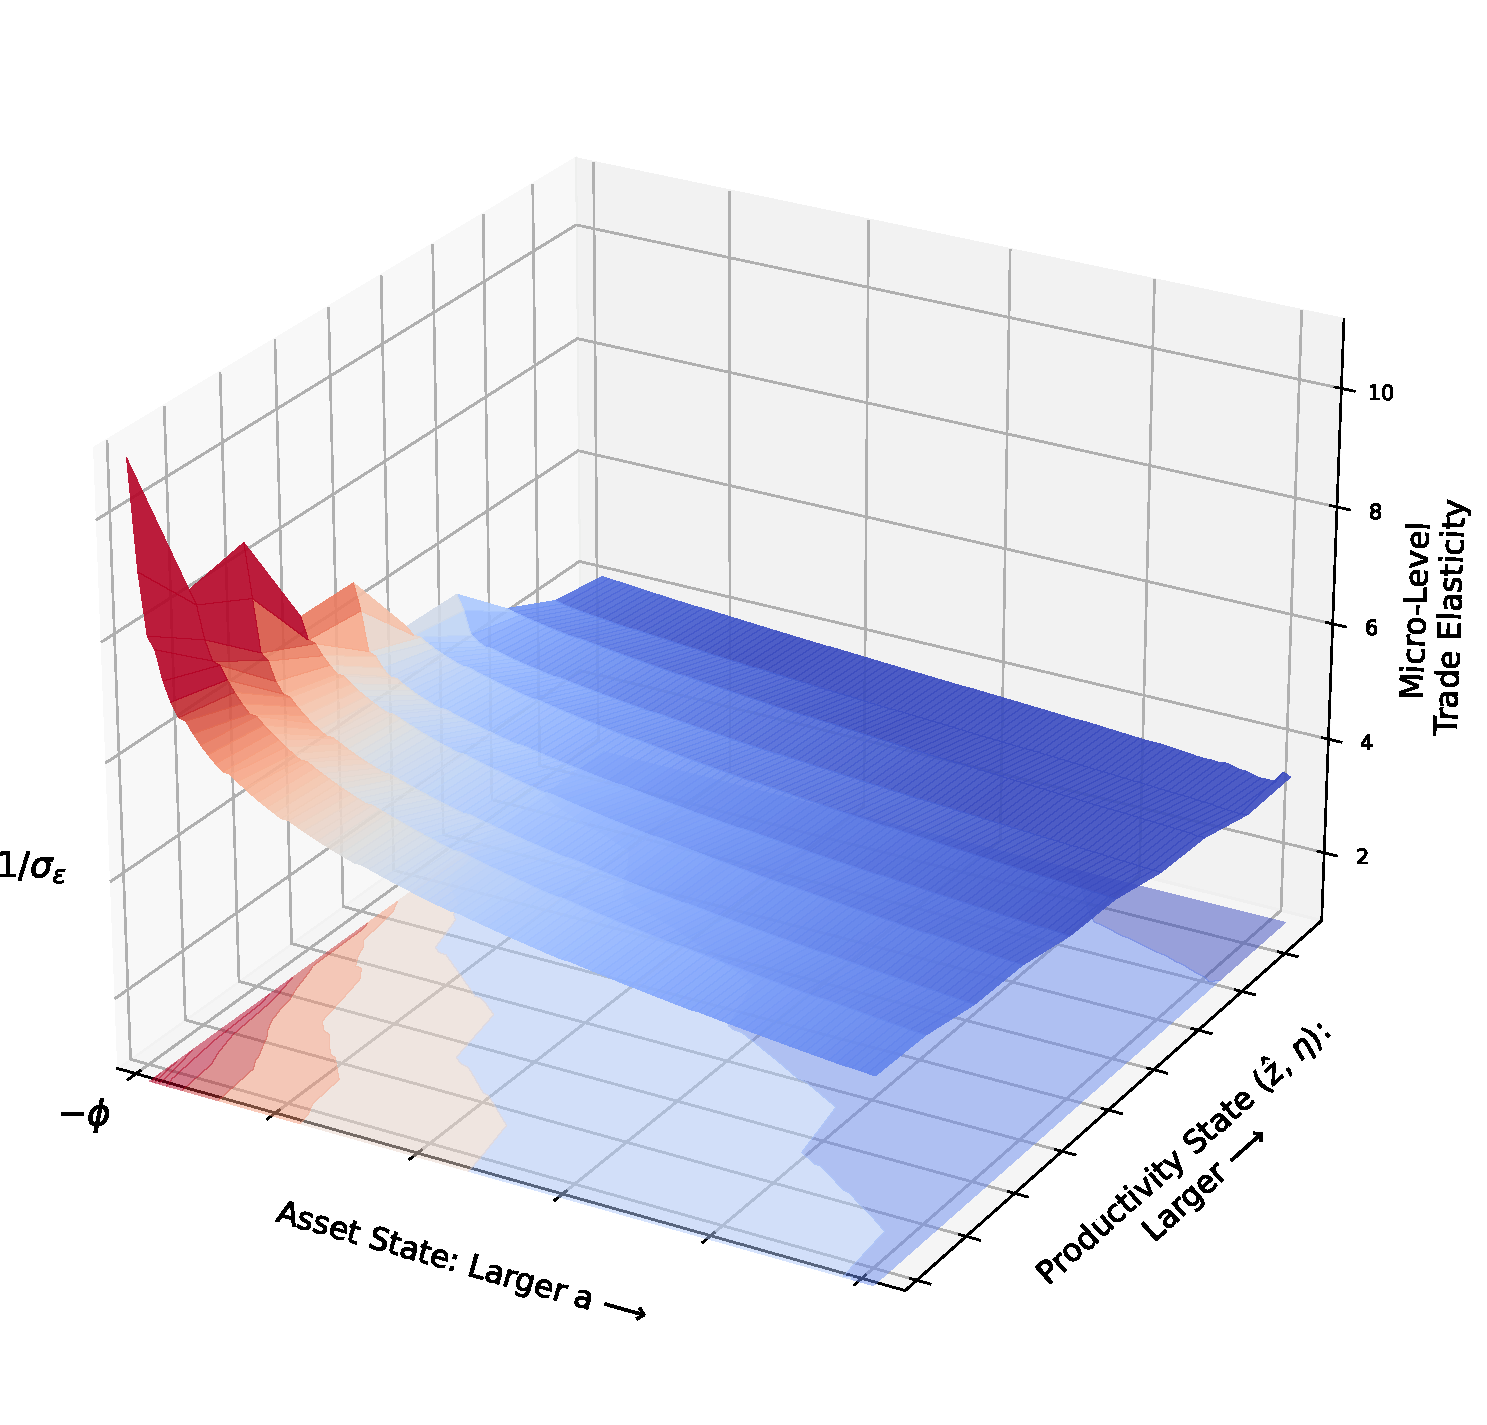
\includegraphics[scale = 0.5]{../notes/figures/micro-elasticity.pdf}}
\end{figure}
\end{frame}


\begin{frame}[t]{Trade Shares: $M_{ij}(a,z) / M_{ii}(a,z)$, by HH-Level State}
\vspace{-.5cm}
\begin{figure}[t]
\centerline{
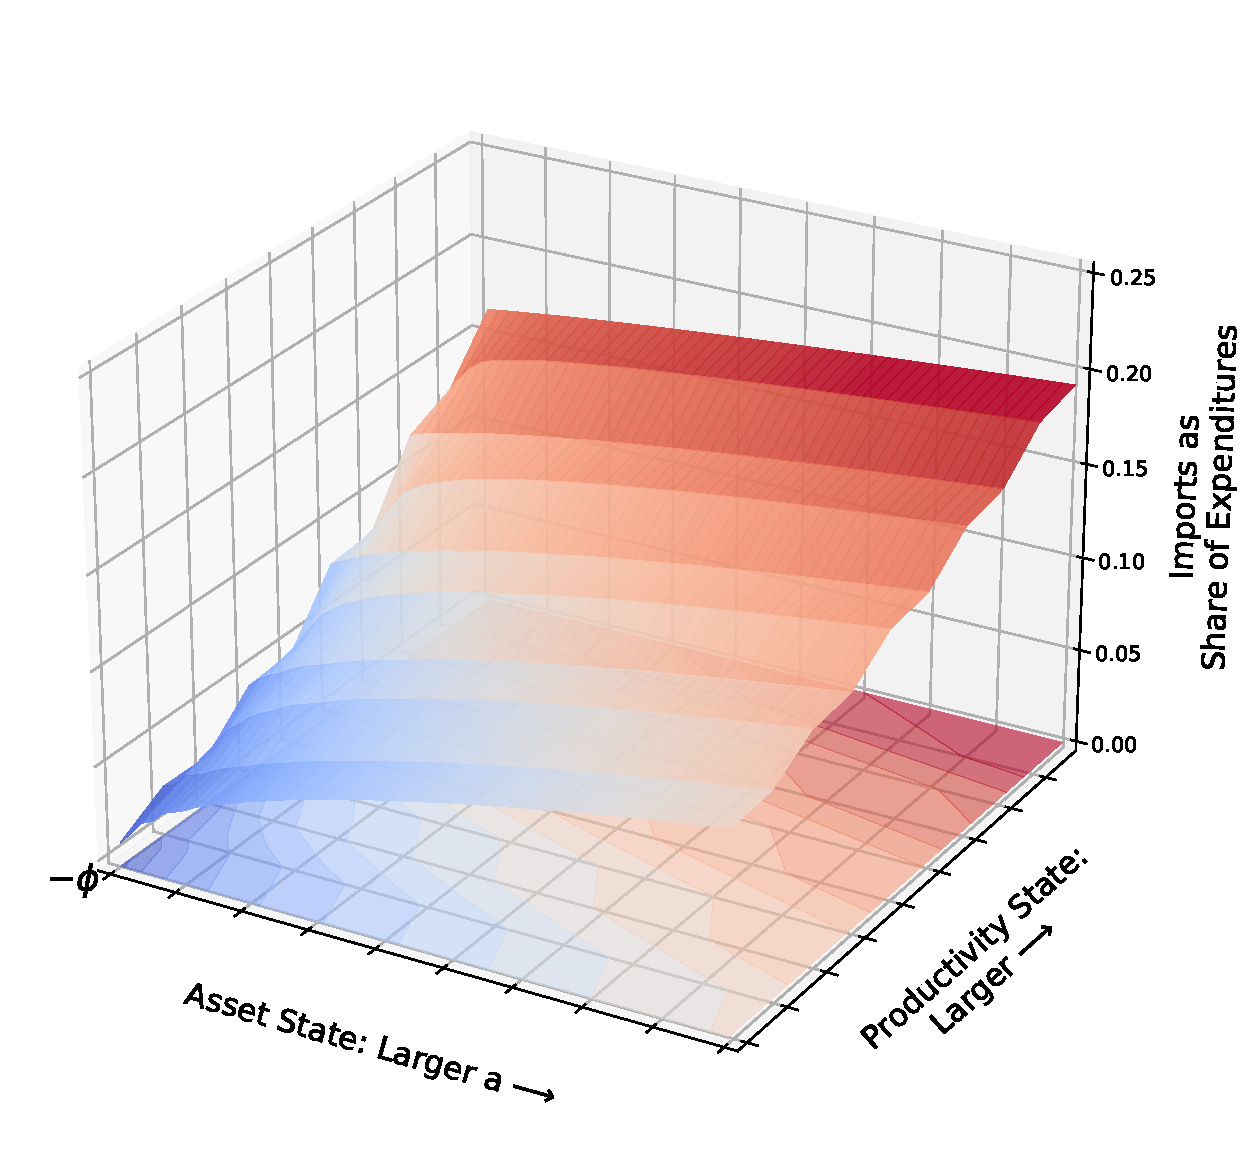
\includegraphics[scale = 0.5]{../notes/figures/trade-share.pdf}}
\end{figure}
\end{frame}


\begin{frame}[t]{H-A Gains from Trade}
\smallskip
\textbf{Proposition \#2: H-A Welfare Gains from Trade.} The gains from trade under a utilitarian social welfare function are
\begin{align*}
\frac{\mathrm{d} W_{i}}{\mathrm{d} d_{ij} / d_{ij}} \approx \int_{z} \int_{a}  \bigg \{ \underbrace{\frac{\mathrm{d} v_i(a, z)}{\mathrm{d} d_{ij} / d_{ij}}}_{\small \mbox{gains to hh}}  + \underbrace{v_{i}(a,z) \frac{\mathrm{d} \lambda_{i}(a,z)/ \lambda_{i}(a,z)}{\mathrm{d} d_{ij} / d_{ij}}}_{\small \mbox{gains to reallocation}}   \bigg \} L_i \lambda_{i}(a,z),
\nonumber
\end{align*}
where $v_i$ is value function before realization of taste shocks; $\approx$ is about abstracting from transition. \\
\medskip
Household-level gains are
\begin{align*}
\frac{\mathrm{d} v_i(a, z)}{\mathrm{d} d_{ij} / d_{ij}} \approx \mathbb{E}_{z} \sum_{t = 0}^{\infty} \beta^{t} \bigg \{ -\sigma_{\epsilon} \frac{\mathrm{d} \pi_{ii}(a_{t},z_{t}) / \pi_{ii}(a_{t},z_{t})}{\mathrm{d}d_{ij} / d_{ij}} + u'(c_{ii}(a_{t},z_{t}))a_{t} \frac{\mathrm{d} R_{i}}{\mathrm{d} d_{ij} / d_{ij}} \bigg \}.
\end{align*}\\
\bigskip
\medskip
HH-level gains pick up two effects:
\begin{itemize}
\item An ACR-like term reflecting how it's home choice changes\ldots basically the gains from substitution.
\smallskip
\item How hh's wealth ($+$ or $-$) changes through GE effects on interest rates.
\end{itemize}
\end{frame}

%%%%%%%%%%%%%%%%%%%%%%%%%%%%%%%%%%%%%%%%%%%%%%%%%%%%%%%%%%%%%%%%%%%%%%%%%%%%%%%%%%%%%%%%%%%%%%%%
%%%%%%%%%%%%%%%%%%%%%%%%%%%%%%%%%%%%%%%%%%%%%%%%%%%%%%%%%%%%%%%%%%%%%%%%%%%%%%%%%%%%%%%%%%%%%%%%

\begin{frame}[t]{H-A Gains from Trade: $\log$ Preferences $\Rightarrow$ Separation of Trade and Heterogeneity}
\smallskip
\textbf{Proposition \#3: Separation of Trade and Micro-Heterogeneity.} In the dynamic, heterogenous agent trade model where preferences are logarithmic over the physical commodity
\begin{align}
\tilde{u}( c_{ijt}, \epsilon_{jt} ) =  \log(c_{ijt}) + \epsilon_{jt}, \nonumber
\end{align}
the trade elasticity is
\begin{align}
\theta = -\frac{1}{\sigma_{\epsilon}}, \nonumber
\end{align}
and is independent of household heterogeneity. And the welfare gains from trade are
\begin{align}
\frac{\mathrm{d} W_{i}}{\mathrm{d} d_{ij} / d_{ij}} = -\frac{1}{\theta (1-\beta)} \times \frac{\mathrm{d} \pi_{ii} / \pi_{ii}}{\mathrm{d}d_{ij} / d_{ij}}. \nonumber
\end{align}
and is (i) independent of the household heterogeneity and (ii) summarized by the trade elasticity and the change in the home choice probability (and home share).\\
\bigskip
\medskip
Mimics the results of \citet{anderson1987ces} and \citet{arkolakis2012new}| but stronger in the sense that this is a far more complex economy, i.e. borrowing constraints, risk, and incomplete markets.
\end{frame}

%%%%%%%%%%%%%%%%%%%%%%%%%%%%%%%%%%%%%%%%%%%%%%%%%%%%%%%%%%%%%%%%%%%%%%%%%%%%%%%%%%%%%%%%%%%%%%%%
%%%%%%%%%%%%%%%%%%%%%%%%%%%%%%%%%%%%%%%%%%%%%%%%%%%%%%%%%%%%%%%%%%%%%%%%%%%%%%%%%%%%%%%%%%%%%%%%

\begin{frame}[t]{H-A Trade under Efficiency}
\smallskip
\textbf{Proposition \#4: The Centralized (Efficient) Allocation.} The allocation satisfying the Centralized Planning Problem (with a utilitarian social welfare function) is:\\
\bigskip
\textbf{1.} An allocation of consumption satisfying:
\begin{align}
u'(c_{ij}(z,t) ) = \chi_{j}(t) d_{ij} \nonumber
\end{align}
where $\chi_{j}(t)$ is the multiplier on $j$ resource constraint for variety $j$,\\
\bigskip
\medskip
\textbf{2.} And variety choice probabilities:
\begin{align}
\displaystyle \pi_{ij}(t) =\exp \left( \frac{u(c_{ij}(t)) - u'(c_{ij}(t))c_{ij}(t)}{\sigma_{\epsilon}}\right) \bigg / \sum_{j'}\exp \left( \frac{u(c_{ij'}(t)) - u'(c_{ij'}(t))c_{ij'}(t)}{\sigma_{\epsilon}} \right). \nonumber
\end{align}\\
\bigskip
\medskip
\textbf{1.} is a \citet{backus1993}-like condition. \\
\smallskip
\textbf{2.} is new | trade should reflect the net social benefit of buying that commodity.
\end{frame}
%%%%%%%%%%%%%%%%%%%%%%%%%%%%%%%%%%%%%%%%%%%%%%%%%%%%%%%%%%%%%%%%%%%%%%%%%%%%%%%%%%%%%%%%%%%%%%%%
%%%%%%%%%%%%%%%%%%%%%%%%%%%%%%%%%%%%%%%%%%%%%%%%%%%%%%%%%%%%%%%%%%%%%%%%%%%%%%%%%%%%%%%%%%%%%%%%

\begin{frame}[t]{H-A Gains from Trade under Efficiency}
\smallskip
\textbf{Proposition \#5: Trade Elasticities and Welfare Gains in the Efficient Allocation} The trade elasticity between $i,j$ in the efficient allocation is:
\begin{align}
\theta_{ij} =  -\frac{1}{\sigma_{\epsilon}} \bigg [ u'(c_{ij}) c_{ij} \bigg]. \nonumber
\end{align}\\
\bigskip
And the welfare gains from a reduction in trade costs between $i,j$ are
\begin{align}
\frac{\mathrm{d} W}{\mathrm{d} d_{ij} / d_{ij}} = \frac{\partial W}{\partial d_{ij} / d_{ij}} = \frac{1}{1-\beta} \times u'(c_{ij}) c_{ij} \pi_{ij} L_i, \nonumber
\end{align}
which is the discounted, direct effect from relaxing the resource constraint.\\
\bigskip
\medskip
Mimics the results of \citet{AtkesonBurstein2010} but with household (not firm) heterogeneity. With $\log$ preferences the direct effect is equivalent to \citet{arkolakis2012new}.\\
\bigskip

\end{frame}

%%%%%%%%%%%%%%%%%%%%%%%%%%%%%%%%%%%%%%%%%%%%%%%%%%%%%%%%%%%%%%%%%%%%%%%%%%%%%%%%%%%%%%%%%%%%%%%%
%%%%%%%%%%%%%%%%%%%%%%%%%%%%%%%%%%%%%%%%%%%%%%%%%%%%%%%%%%%%%%%%%%%%%%%%%%%%%%%%%%%%%%%%%%%%%%%%

\begin{frame}[t]{Quantitative Analysis}
\smallskip
Still preliminary. This is what I'm going to do:
\begin{itemize}
  \item Grab trade costs and productivity estimates from 19 country world of \citet{eaton2002technology} and compute an equilibrium.
\smallskip
  \item Explore bilateral reduction in trade costs...I'll explain in two slides.
\end{itemize}
\bigskip
Other important parameters and how I set them for today.
\begin{itemize}
\item Taste shock parameter so $1 / \sigma_{\epsilon} = 4.0$. CRRA for $u$ with relative risk aversion $= 1.5$.
\smallskip
\item Earnings process is a mixture of a persistent and transitory component and calibrated as in\\ \citet*{krueger2016macroeconomics}.
\smallskip
\item Borrowing constraint is set $\approx 2\times$ earnings for US. Discount factor set so $R \approx$ 2\% for US.
\end{itemize}
\end{frame}
%%%%%%%%%%%%%%%%%%%%%%%%%%%%%%%%%%%%%%%%%%%%%%%%%%%%%%%%%%%%%%%%%%%%%%%%%%%%%%%%%%%%%%%%%%%%%%%%
%%%%%%%%%%%%%%%%%%%%%%%%%%%%%%%%%%%%%%%%%%%%%%%%%%%%%%%%%%%%%%%%%%%%%%%%%%%%%%%%%%%%%%%%%%%%%%%%

\begin{frame}[t]{Bilateral Trade: Model vs. Data}
\begin{figure}[!t]
\centering{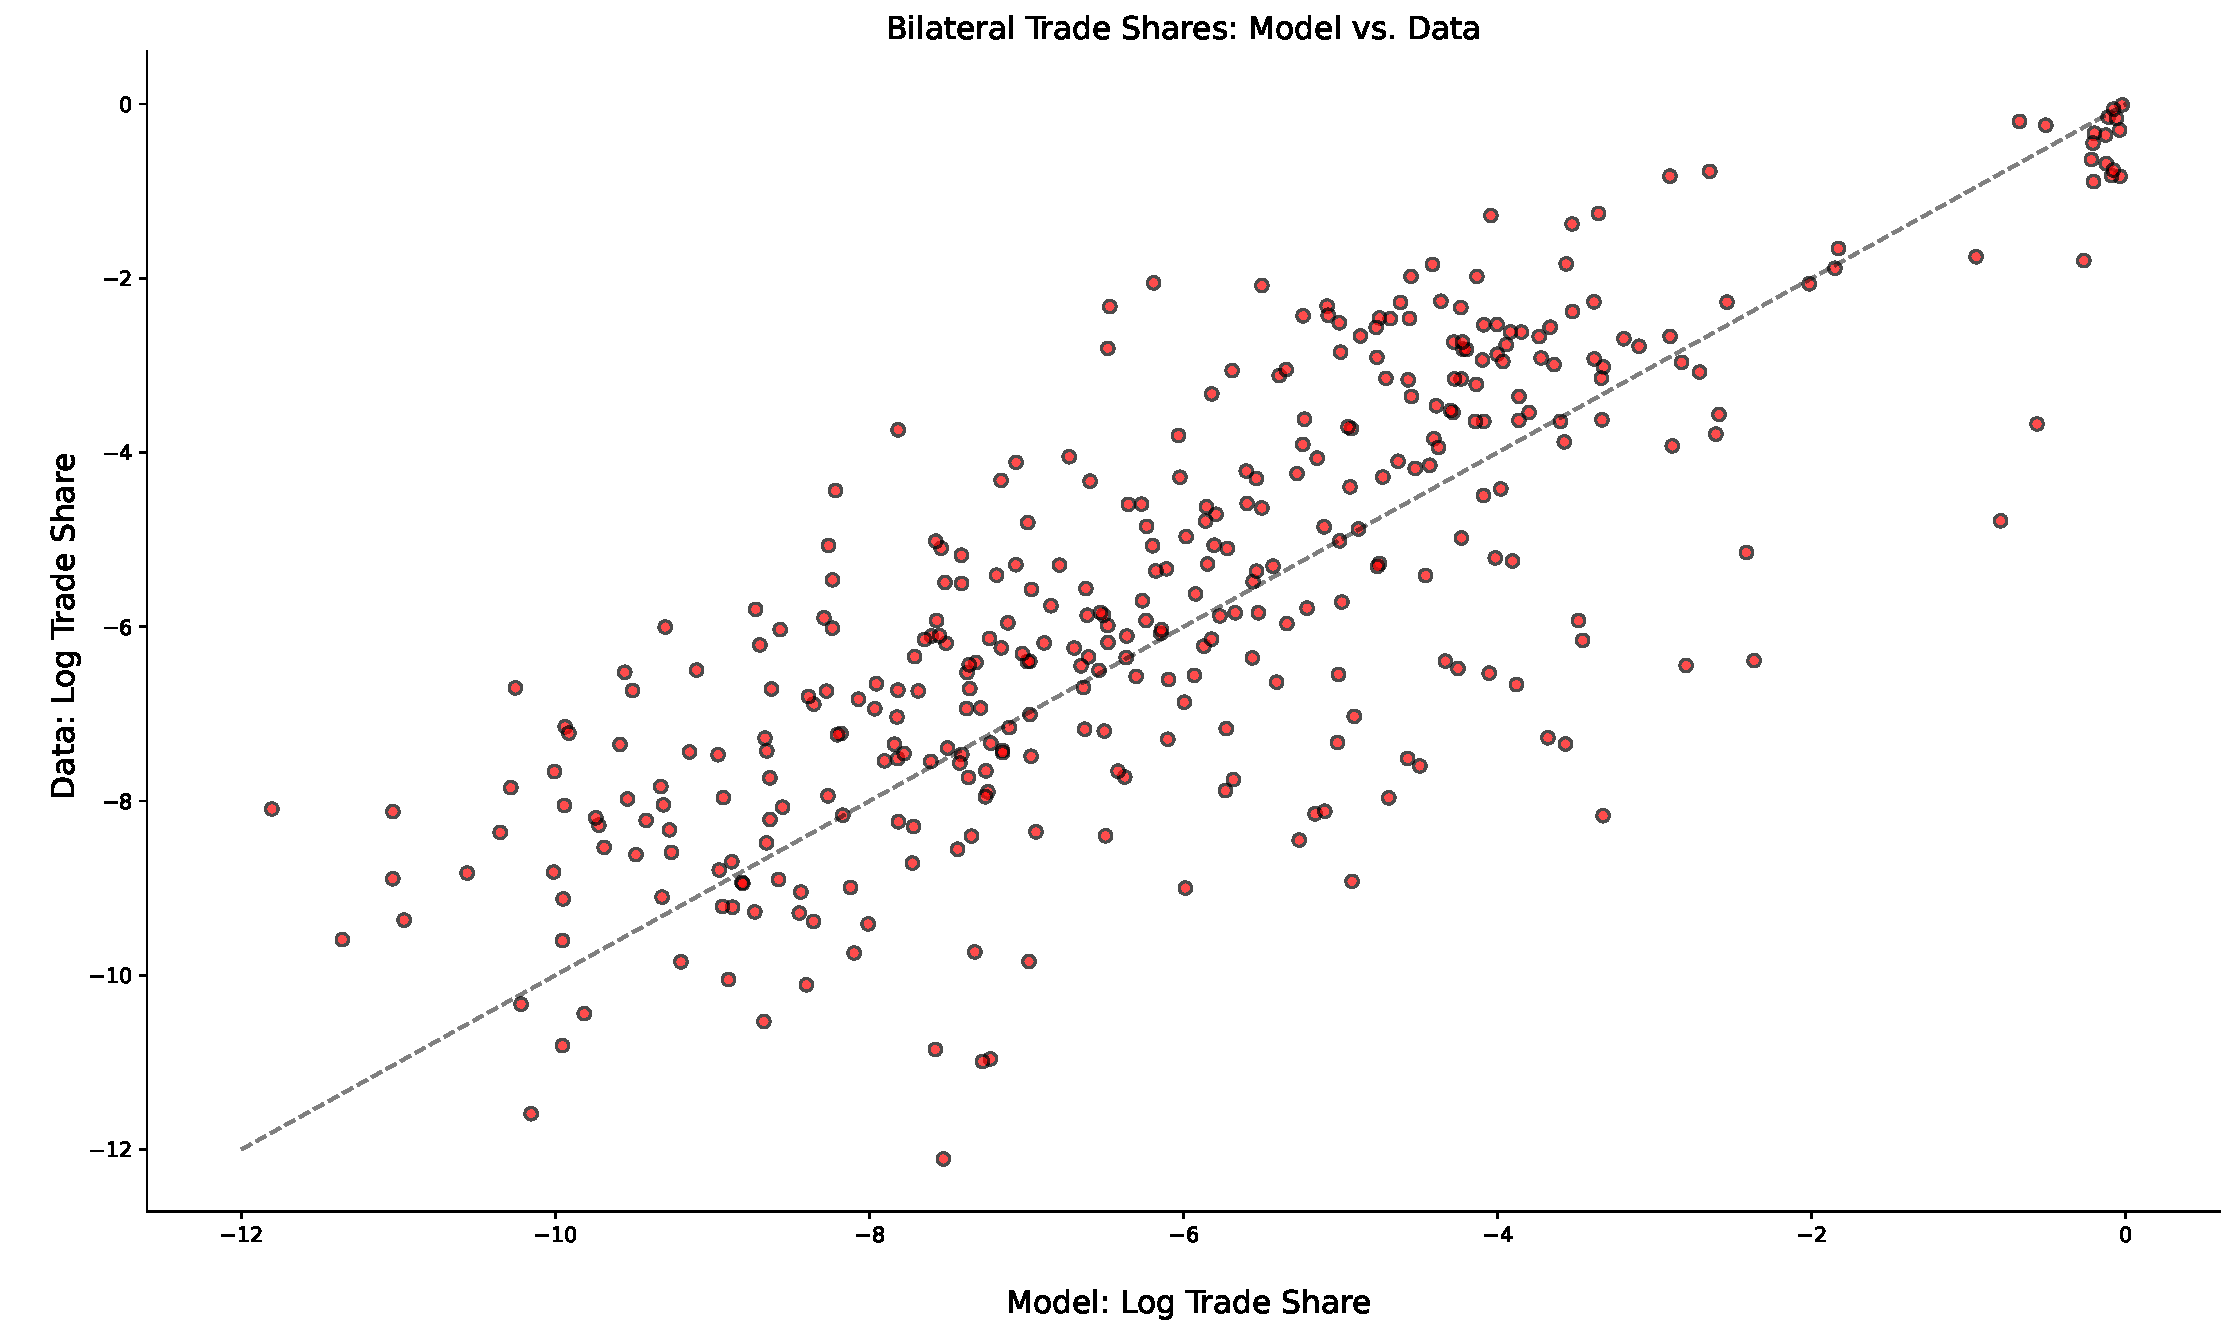
\includegraphics[scale = .35]{../notes/figures/trade-fit.pdf}}
\end{figure}
\end{frame}

%%%%%%%%%%%%%%%%%%%%%%%%%%%%%%%%%%%%%%%%%%%%%%%%%%%%%%%%%%%%%%%%%%%%%%%%%%%%%%%%%%%%%%%%%%%%%%%%
%%%%%%%%%%%%%%%%%%%%%%%%%%%%%%%%%%%%%%%%%%%%%%%%%%%%%%%%%%%%%%%%%%%%%%%%%%%%%%%%%%%%%%%%%%%%%%%%

\begin{frame}[t]{Taking the Model for a Ride}
\smallskip
Two ideas I want to illustrate:\\
\medskip
\textbf{1.} \textbf{You pick the market, you pick a person.}
\begin{itemize}
  \item Rich vs. poor benefit differently depending upon the market.
\end{itemize}
\bigskip
\textbf{2.} \textbf{Modern day Stolper-Samuelson.}
\begin{itemize}
\item Who directly benefits from \textbf{1.} effects $R$ $\Rightarrow$ shapes the extent to which their are winners and losers.
\end{itemize}
\bigskip
Next slides: 10\% reduction to US import trade cost on different source markets\ldots Japan, Canada. Focus on US welfare and break it down by
\begin{itemize}
\item[A.] Fix $R$ \& $w$, so what is direct effect of change in trade cost,
\smallskip
\item[B.] $R$ \& $w$ adjust to clear goods and asset markets.
\end{itemize}
\end{frame}

%%%%%%%%%%%%%%%%%%%%%%%%%%%%%%%%%%%%%%%%%%%%%%%%%%%%%%%%%%%%%%%%%%%%%%%%%%%%%%%%%%%%%%%%%%%%%%%%
%%%%%%%%%%%%%%%%%%%%%%%%%%%%%%%%%%%%%%%%%%%%%%%%%%%%%%%%%%%%%%%%%%%%%%%%%%%%%%%%%%%%%%%%%%%%%%%%

\begin{frame}[t]{U.S. Trade: 10\% Reduction to Japan, {\color{red} Fixed $R$ \& $w$} }
\begin{figure}[t]
\centering{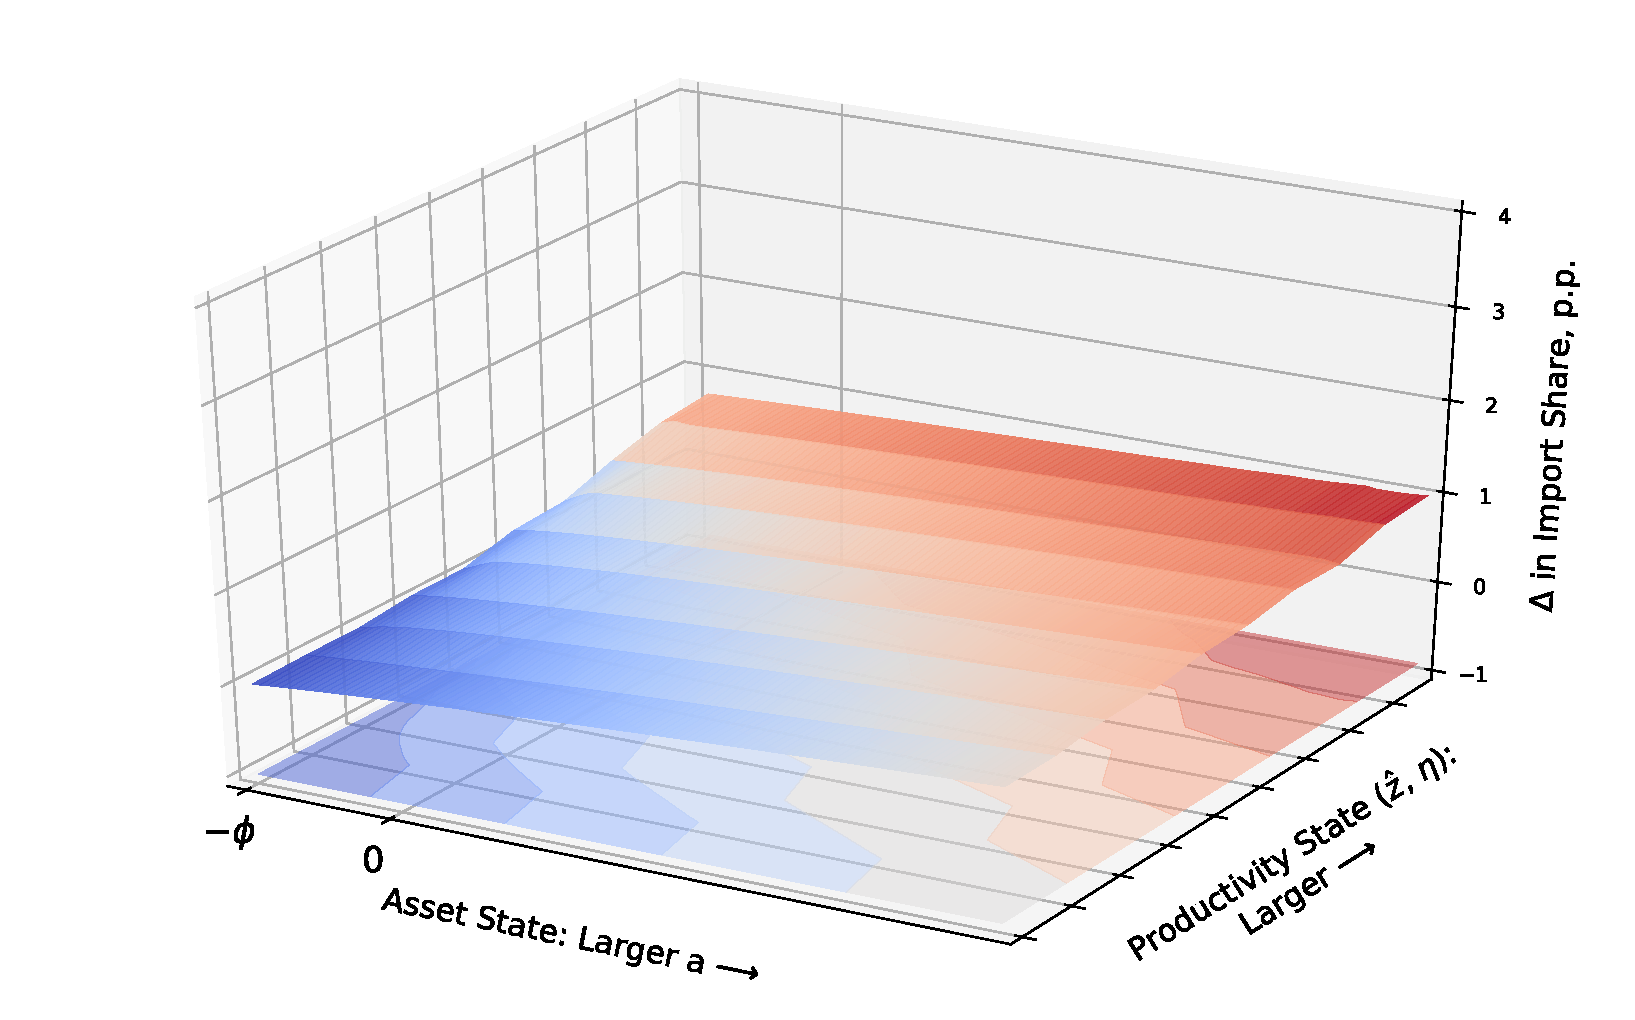
\includegraphics[scale = .45]{../notes/figures/japan-trade.pdf}}
\end{figure}
\end{frame}

\begin{frame}[t]{U.S. Welfare: 10\% Reduction to Japan, {\color{red} Fixed $R$ \& $w$} }
\begin{figure}[!t]
\centering{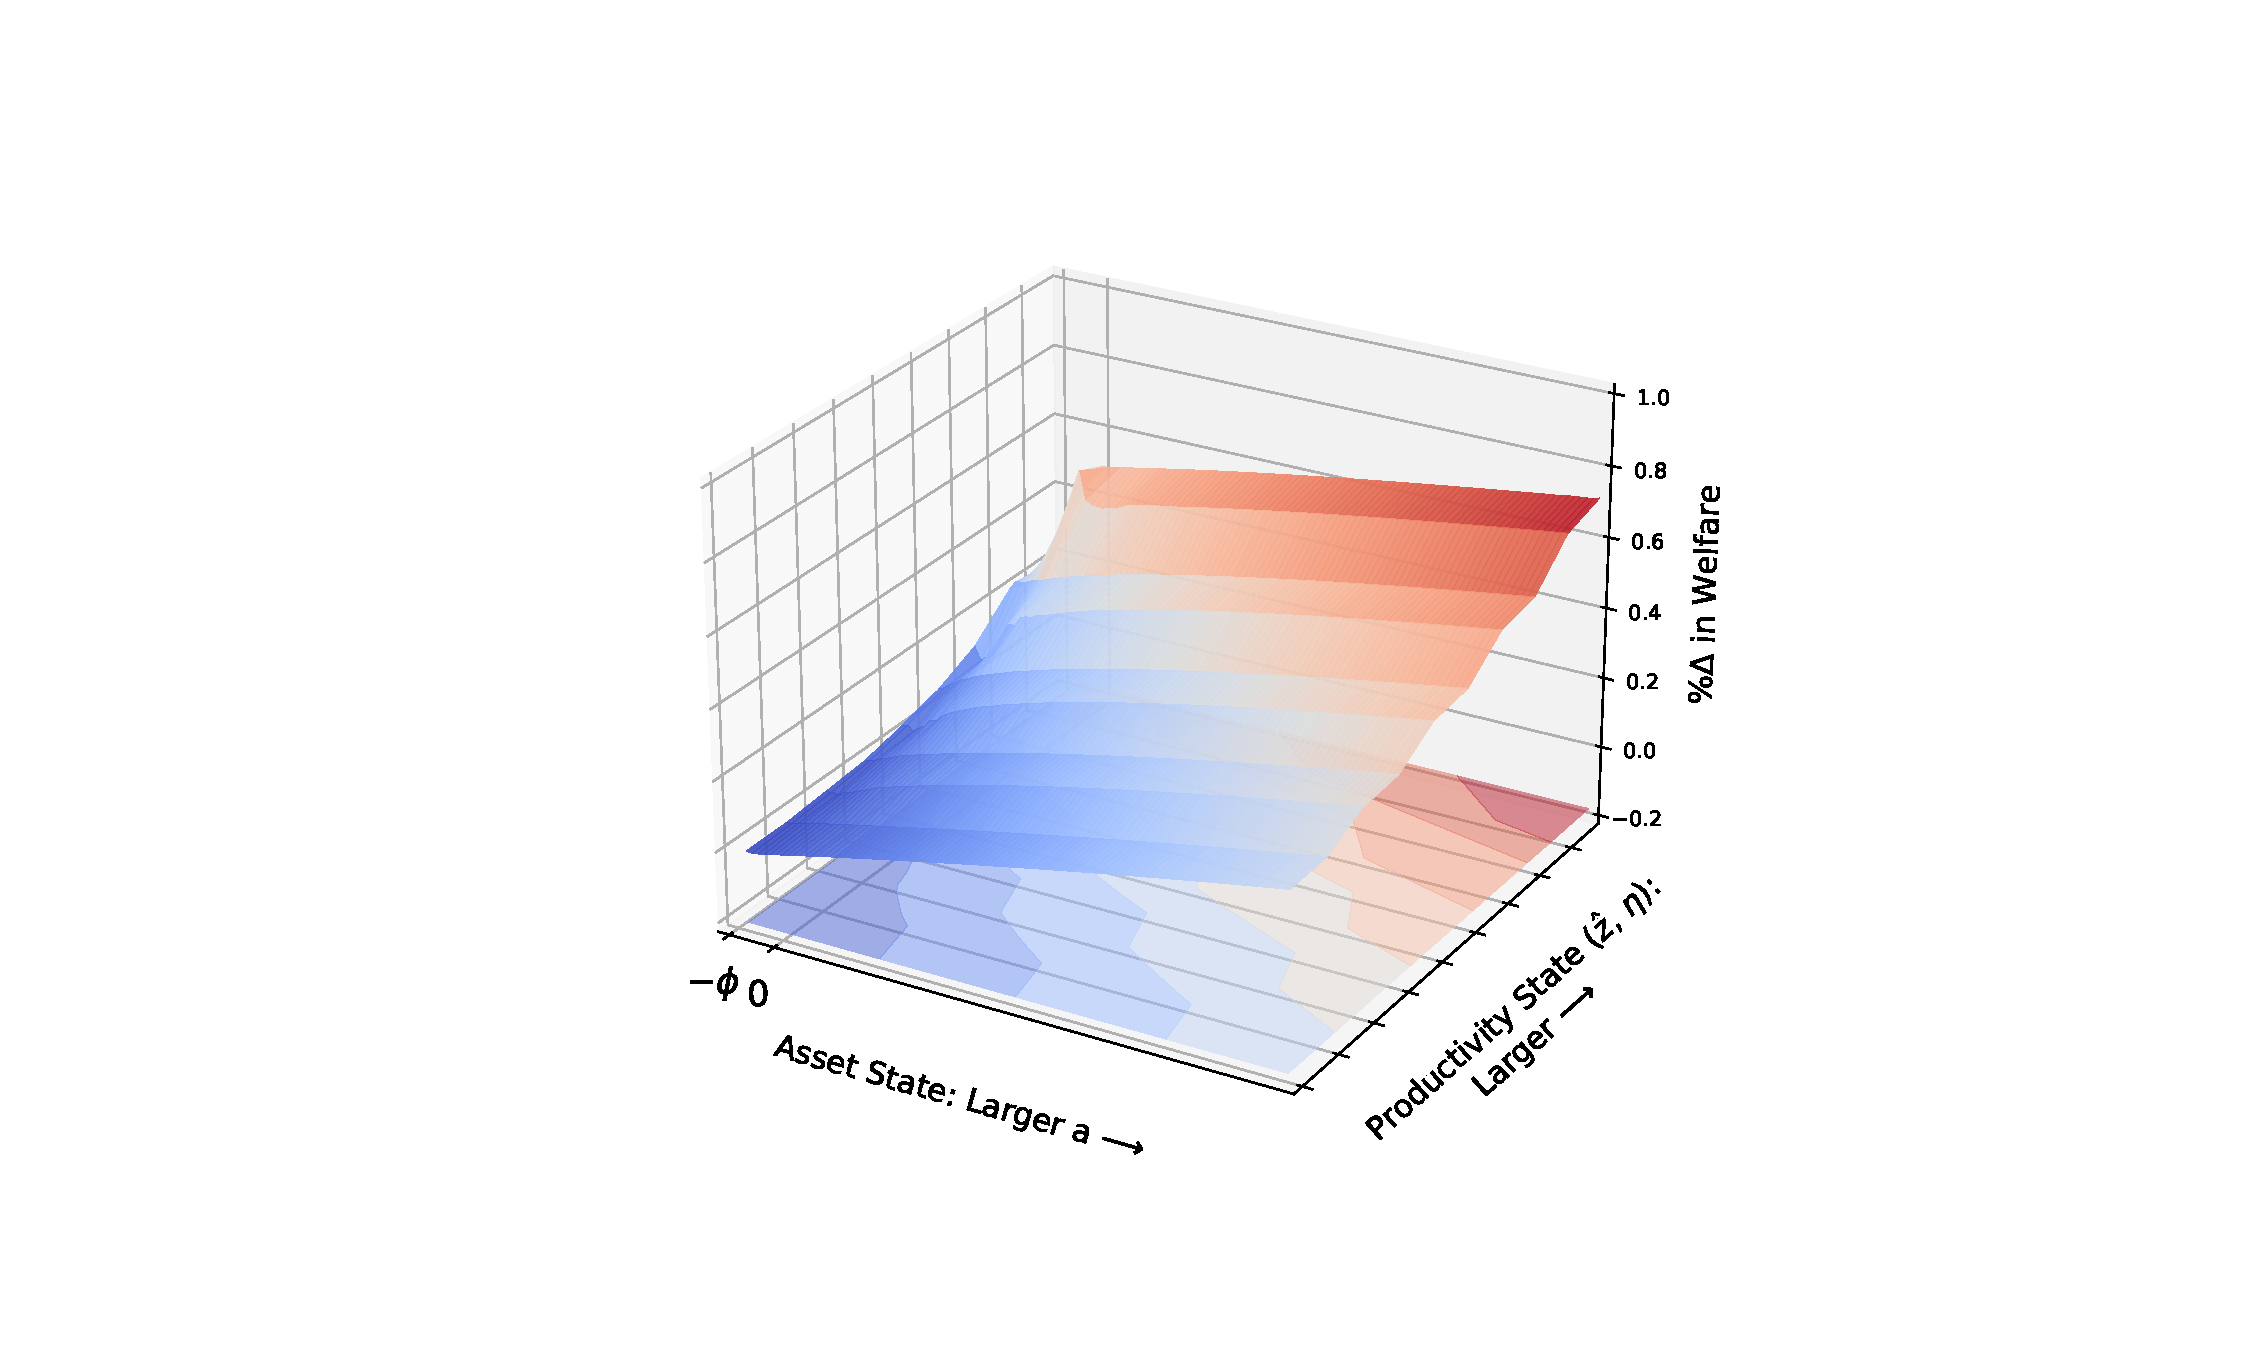
\includegraphics[scale = .45]{../notes/figures/welfare-jpn-fix-p.pdf}}
\end{figure}
\end{frame}

\begin{frame}[t]{U.S. Welfare: 10\% Reduction to Japan, {\color{red} GE} }
\begin{figure}[!t]
\centering{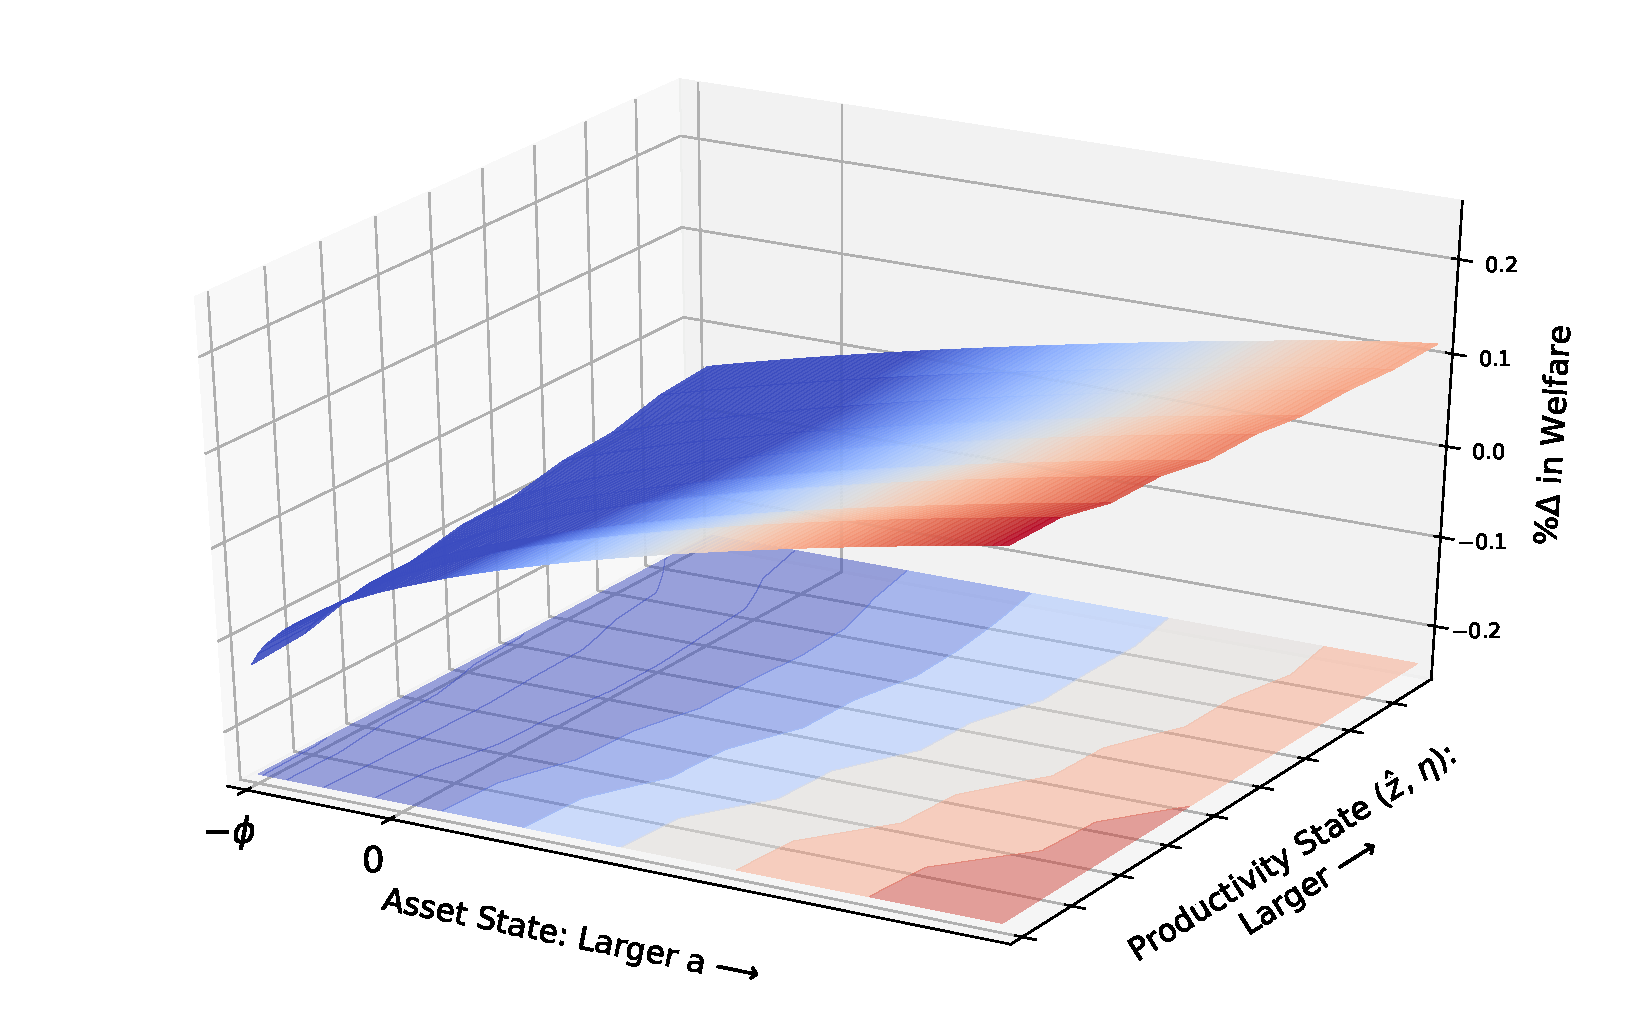
\includegraphics[scale = .45]{../notes/figures/welfare-jpn.pdf}}
\end{figure}
\end{frame}

\begin{frame}[t]
\frametitle{U.S. Welfare: 10\% Reduction to Japan}
\begin{table}[t]
\footnotesize
\setlength {\tabcolsep}{6.05mm}
\renewcommand{\arraystretch}{1.80}
\begin{center}
\begin{tabular}{l c c}
\multicolumn{3}{c}{\small \textbf{Welfare by Wealth --- Japan {\color{red} 10\%} Reduction}}\\
\hline
\hline
& \footnotesize  Fixed $R$ \& $w$ & GE: Prices Adjust \\
\cmidrule(lr){2-2}  \cmidrule(lr){3-3}
\footnotesize  Asset Quartile & \footnotesize  Welfare (\% Change) & \footnotesize  Welfare (\% Change) \\
\footnotesize  Bottom quartile  & 0.0193 & -0.095 \\
\footnotesize  Median & 0.0306 & -0.052 \\
\footnotesize  Upper quartile  & 0.0535 & 0.030  \\
\footnotesize  Aggregate & 0.0031 & -0.040 \\
\cmidrule(lr){2-2}  \cmidrule(lr){3-3}
\footnotesize  \% losers & 0.0 & 77.8\\
\hline
\end{tabular}
%\parbox[c]{3.65in}{\vspace{.1cm}
%{\footnotesize \textbf{Note:}}}
\end{center}
\end{table}
\end{frame}

%%%%%%%%%%%%%%%%%%%%%%%%%%%%%%%%%%%%%%%%%%%%%%%%%%%%%%%%%%%%%%%%%%%%%%%%%%%%%%%%%%%%%%%%%%%%%%%%
%%%%%%%%%%%%%%%%%%%%%%%%%%%%%%%%%%%%%%%%%%%%%%%%%%%%%%%%%%%%%%%%%%%%%%%%%%%%%%%%%%%%%%%%%%%%%%%%

\begin{frame}[t]{U.S. Trade: 10\% Reduction to Canada, {\color{red} Fixed $R$ \& $w$} }

\begin{figure}[t]
\centering{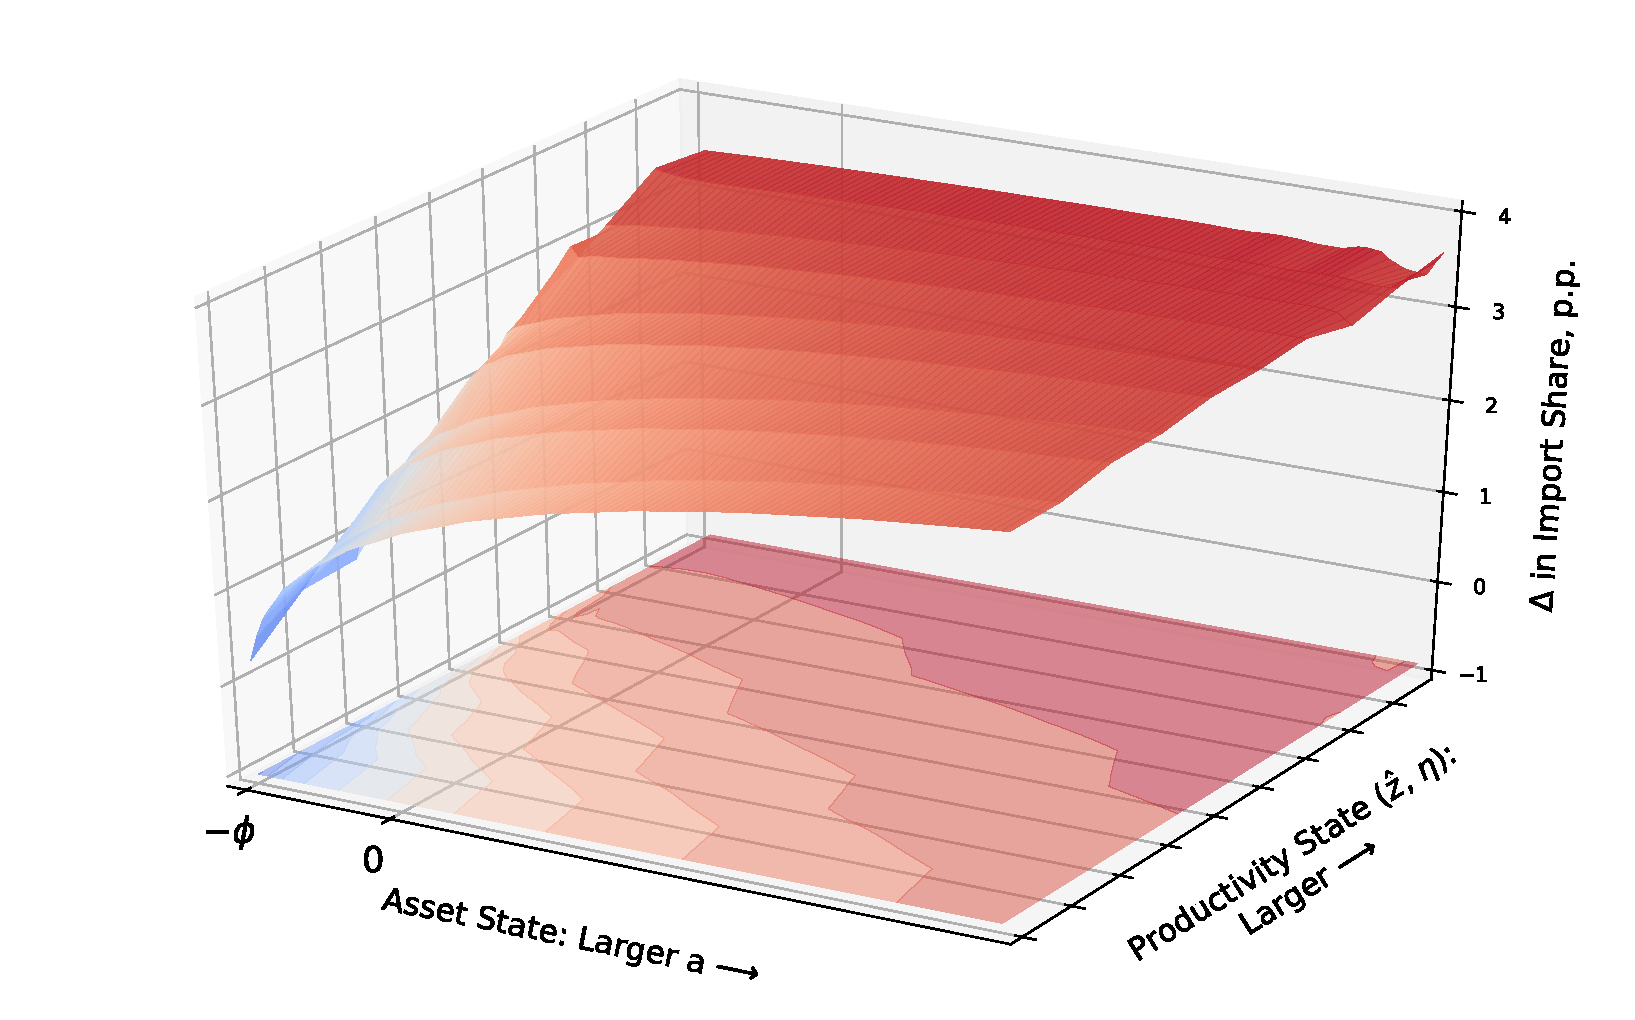
\includegraphics[scale = .45]{../notes/figures/canada_trade.pdf}}
\end{figure}
\end{frame}


\begin{frame}[t]{U.S. Welfare: 10\% Reduction to Canada, {\color{red} Fixed $R$ \& $w$} }
\begin{figure}[t]
\centering{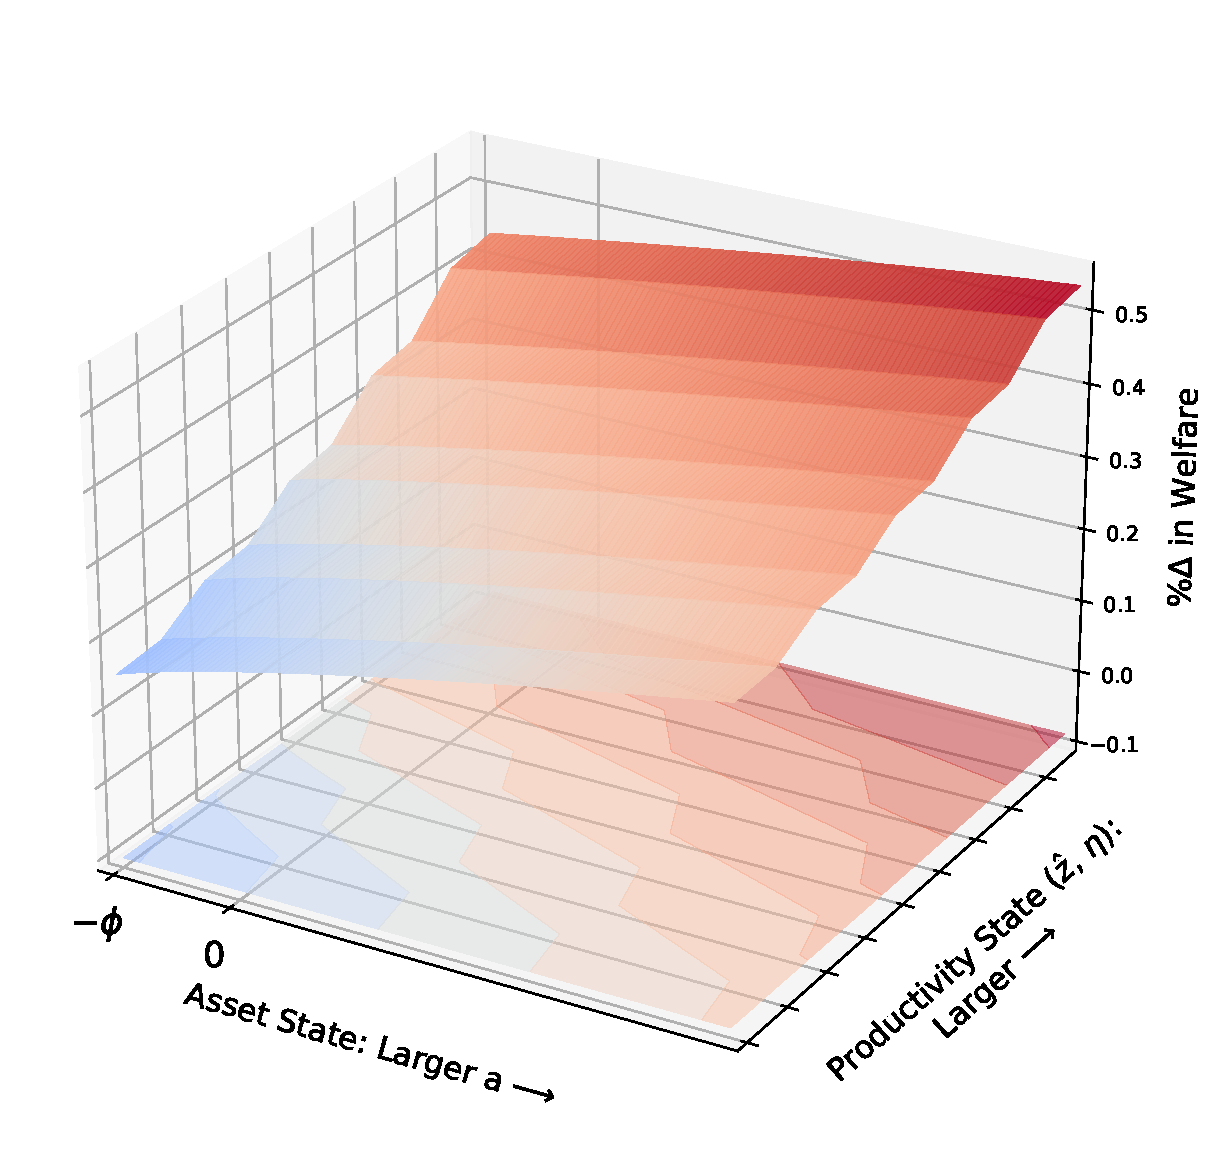
\includegraphics[scale = .45]{../notes/figures/welfare-can-fix-p.pdf}}
\end{figure}
\end{frame}

\begin{frame}[t]{U.S. Welfare: 10\% Reduction to Canada, {\color{red} GE } }
\begin{figure}[!t]
\centering{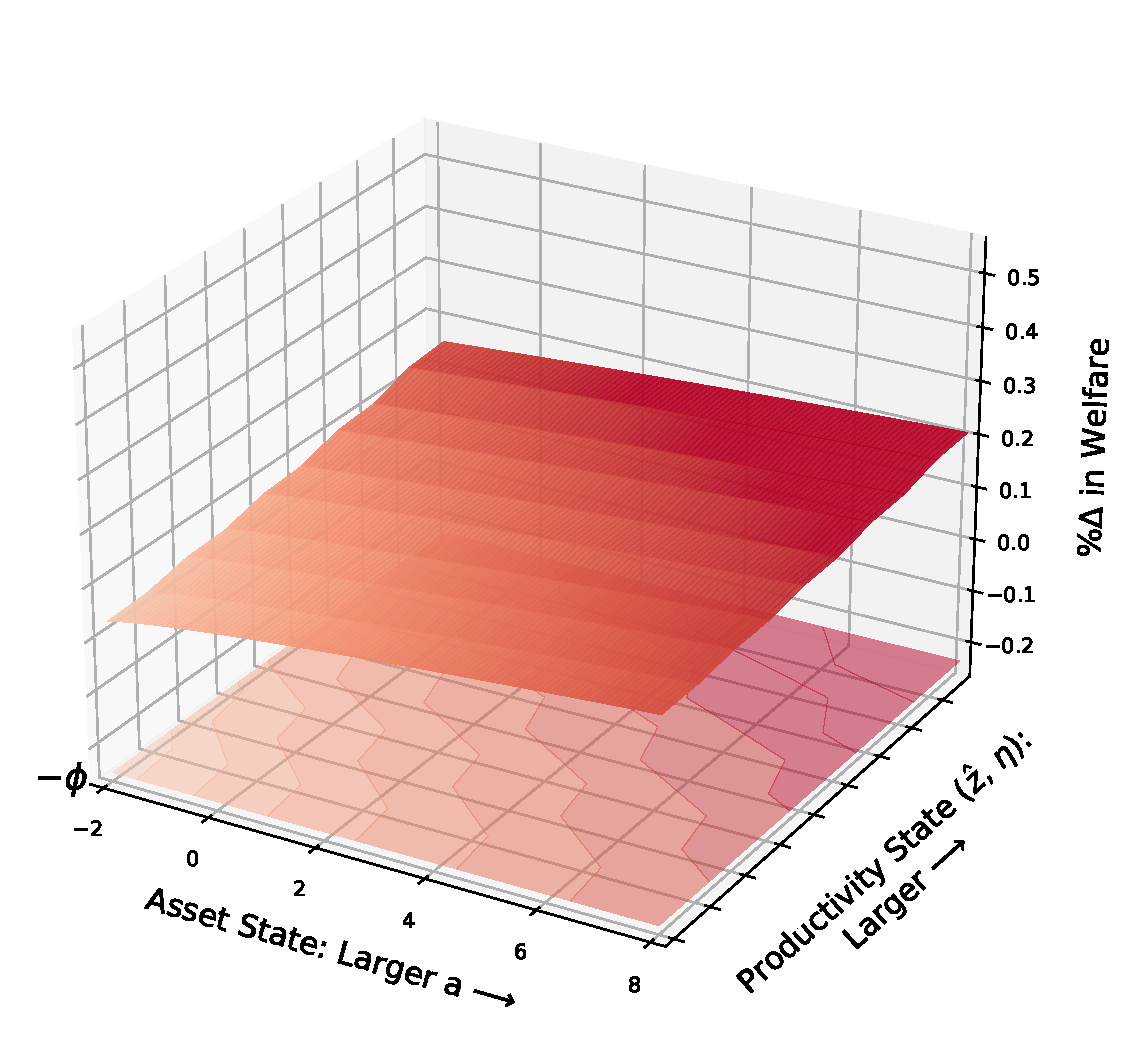
\includegraphics[scale = .45]{../notes/figures/welfare-can.pdf}}
\end{figure}
\end{frame}


\begin{frame}[t]
\frametitle{U.S. Welfare: 10\% Reduction to Canada}
\begin{table}[!t]
\footnotesize
\setlength {\tabcolsep}{6.05mm}
\renewcommand{\arraystretch}{1.80}
\begin{center}
\begin{tabular}{l c c}
\multicolumn{3}{c}{\small \textbf{Welfare by Wealth --- Canada {\color{red} 10\%} Reduction}}\\
\hline
\hline
& \footnotesize  Fixed $R$ \& $w$ & GE: Prices Adjust \\
\cmidrule(lr){2-2}  \cmidrule(lr){3-3}
\footnotesize  Asset Quartile & \footnotesize  Welfare (\% Change) & \footnotesize  Welfare (\% Change) \\
\footnotesize  Bottom quartile  & 0.21 & 0.06 \\
\footnotesize  Median & 0.28 & 0.09 \\
\footnotesize  Upper quartile  & 0.39 & 0.14  \\
\footnotesize  Aggregate & 0.30 &  0.09 \\
\cmidrule(lr){2-2}  \cmidrule(lr){3-3}
\footnotesize  \% losers & 0.0 & 0.0\\
\hline
\end{tabular}
%\parbox[c]{3.65in}{\vspace{.1cm}
%{\footnotesize \textbf{Note:}}}
\end{center}
\end{table}
\end{frame}


%%%%%%%%%%%%%%%%%%%%%%%%%%%%%%%%%%%%%%%%%%%%%%%%%%%%%%%%%%%%%%%%%%%%%%%%%%%%%%%%%%%%%%%%%%%%%%%%
%%%%%%%%%%%%%%%%%%%%%%%%%%%%%%%%%%%%%%%%%%%%%%%%%%%%%%%%%%%%%%%%%%%%%%%%%%%%%%%%%%%%%%%%%%%%%%%%

\begin{frame}[t]
\frametitle{The Planner\ldots}
\smallskip
This idea that the being exposed to some markets is better than others shows up in the planners allocation.\\
\bigskip
Next two slides..
\begin{itemize}
\item Trade in the decentralized equilibrium vs.
\medskip
\item the allocation chosen by the planner
\end{itemize}
\end{frame}


%%%%%%%%%%%%%%%%%%%%%%%%%%%%%%%%%%%%%%%%%%%%%%%%%%%%%%%%%%%%%%%%%%%%%%%%%%%%%%%%%%%%%%%%%%%%%%%%
%%%%%%%%%%%%%%%%%%%%%%%%%%%%%%%%%%%%%%%%%%%%%%%%%%%%%%%%%%%%%%%%%%%%%%%%%%%%%%%%%%%%%%%%%%%%%%%%

\begin{frame}[t]{US Trade in the Decentralized Equilibrium}

\begin{figure}[t]
\centering{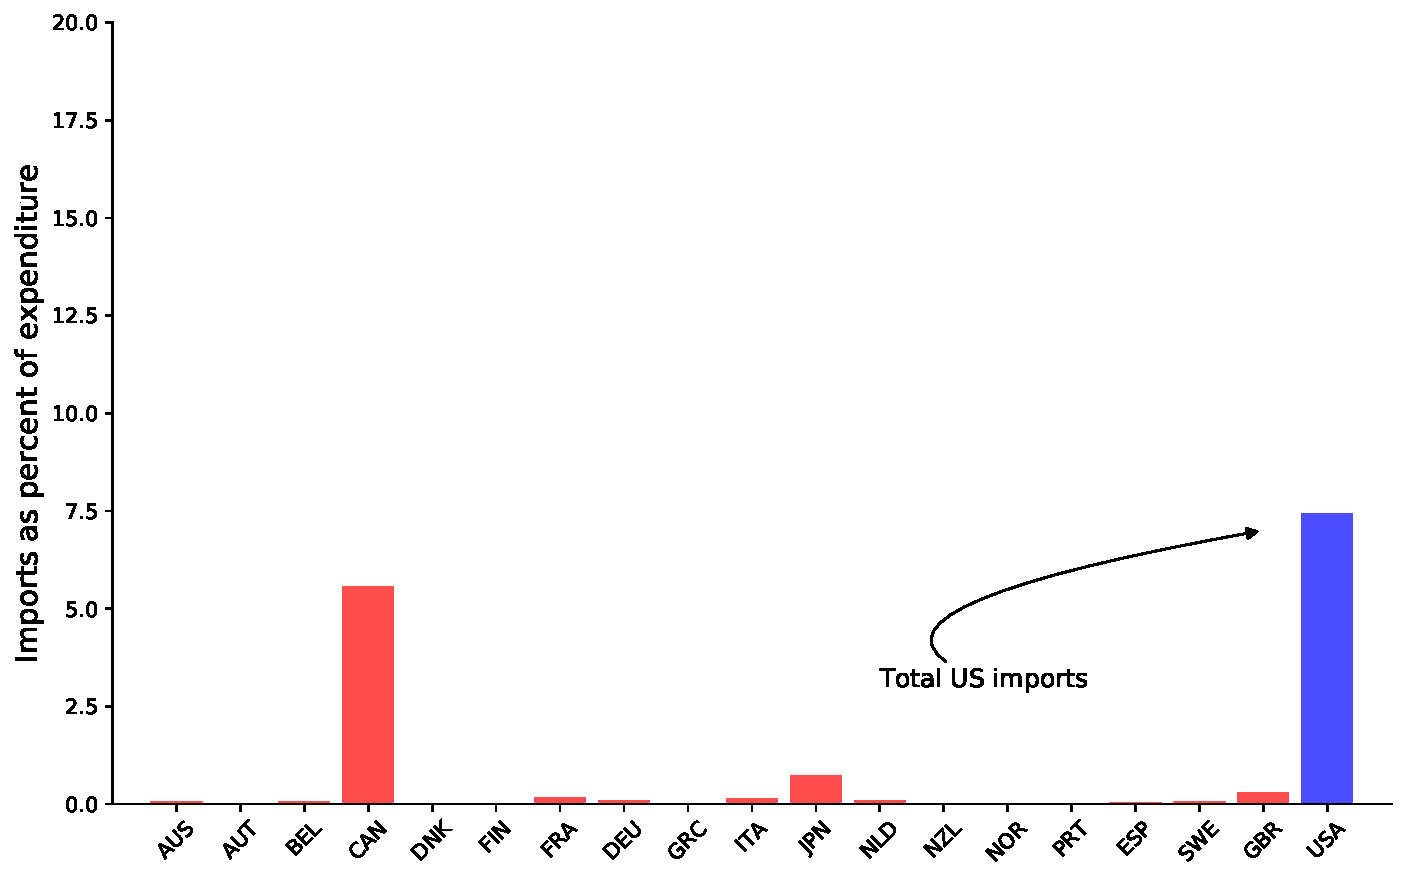
\includegraphics[scale = .55]{../notes/figures/decentralized-trade-us.pdf}}
\end{figure}
\end{frame}

\begin{frame}[t]{US Trade in the Planner's Allocation}

\begin{figure}[t]
\centering{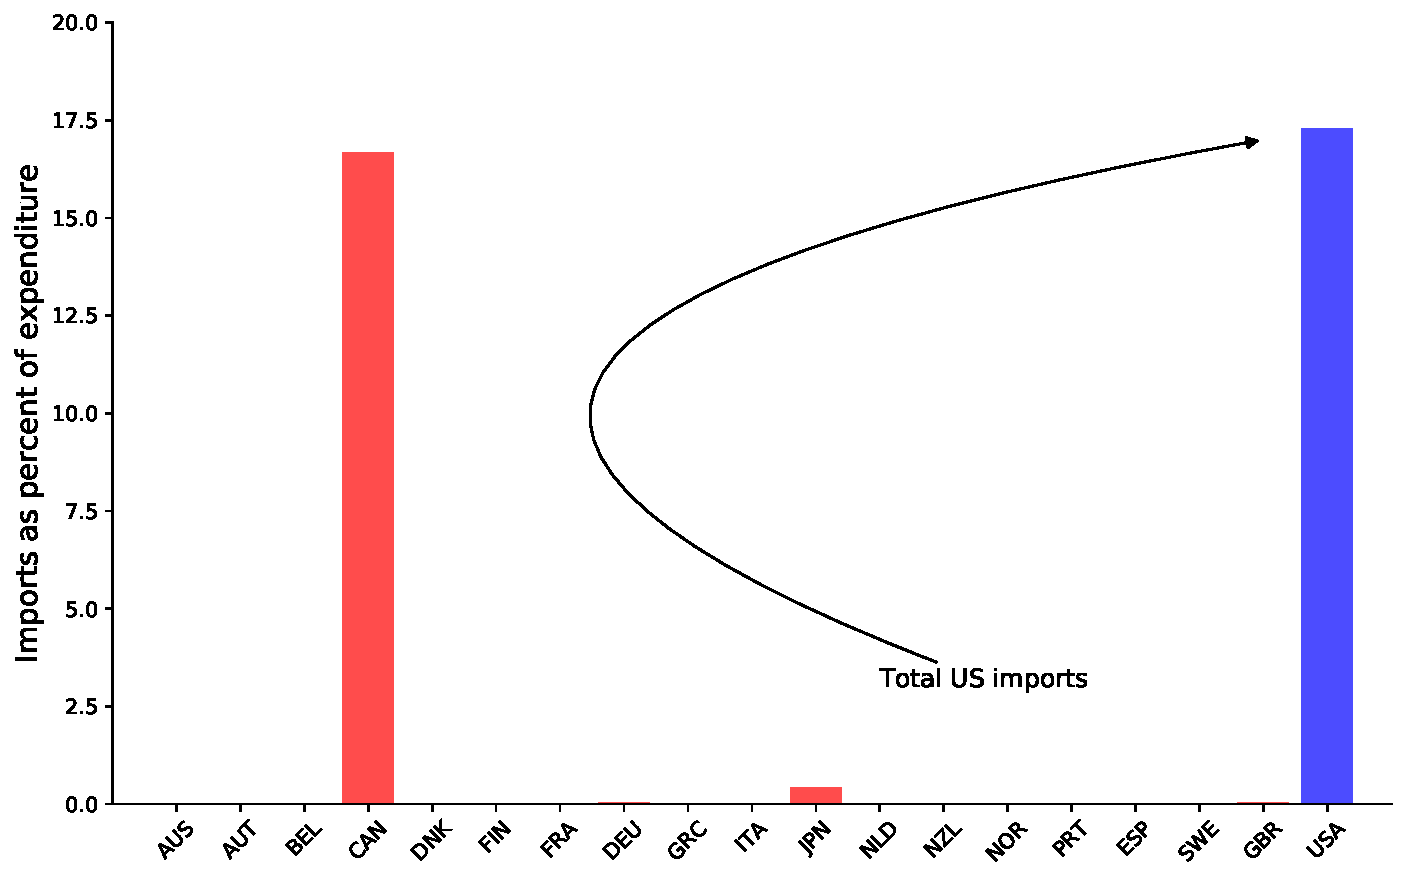
\includegraphics[scale = .55]{../notes/figures/planner-trade-us.pdf}}
\end{figure}
\end{frame}


%%%%%%%%%%%%%%%%%%%%%%%%%%%%%%%%%%%%%%%%%%%%%%%%%%%%%%%%%%%%%%%%%%%%%%%%%%%%%%%%%%%%%%%%%%%%%%%%
%%%%%%%%%%%%%%%%%%%%%%%%%%%%%%%%%%%%%%%%%%%%%%%%%%%%%%%%%%%%%%%%%%%%%%%%%%%%%%%%%%%%%%%%%%%%%%%%

%%%%%%%%%%%%%%%%%%%%%%%%%%%%%%%%%%%%%%%%%%%%%%%%%%%%%%%%%%%%%%%%%%%%%%%%%%%%%%%%%%%%%%%%%%%%%%%%
%%%%%%%%%%%%%%%%%%%%%%%%%%%%%%%%%%%%%%%%%%%%%%%%%%%%%%%%%%%%%%%%%%%%%%%%%%%%%%%%%%%%%%%%%%%%%%%%

\appendix

\newcounter{finalframe}
\setcounter{finalframe}{\value{framenumber}}

\begin{frame}[allowframebreaks]
\frametitle{References}
\scriptsize
\bibliography{../notes/bibtex/micro_price_bibtex}
\end{frame}


\begin{frame}[t]{U.S. Welfare: 10\% Reduction to a Small Market (Australia), {\color{red} Fixed $R$ \& $w$} }
\vspace{-.5cm}
\begin{figure}[!t]
\centering{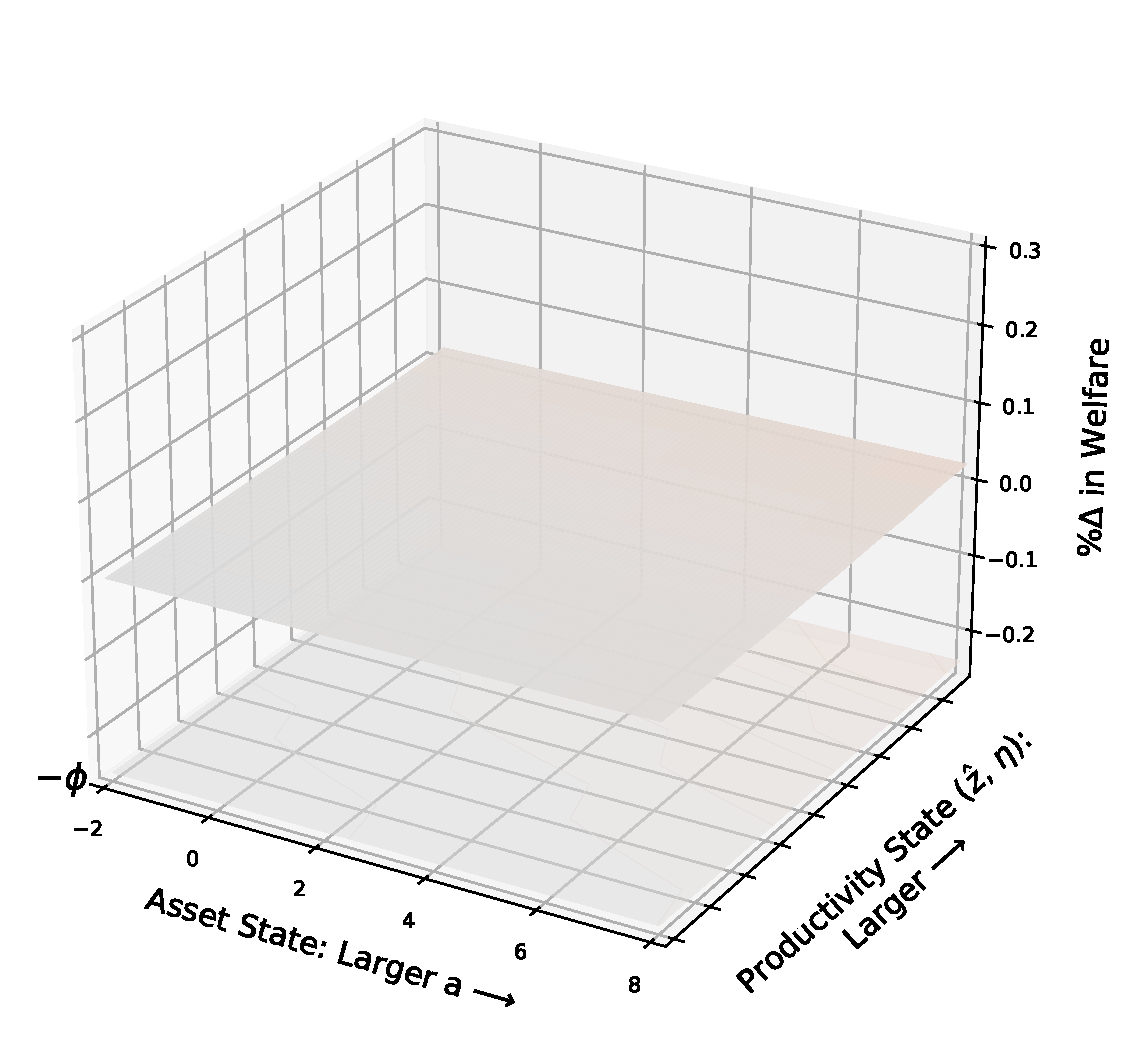
\includegraphics[scale = .45]{../notes/figures/welfare-aut-fix-p.pdf}}
\end{figure}
\end{frame}

\begin{frame}[t]{U.S. Welfare: 10\% Reduction to a Small Market (Australia), {\color{red} GE} }
\vspace{-.5cm}
\begin{figure}[!t]
\centering{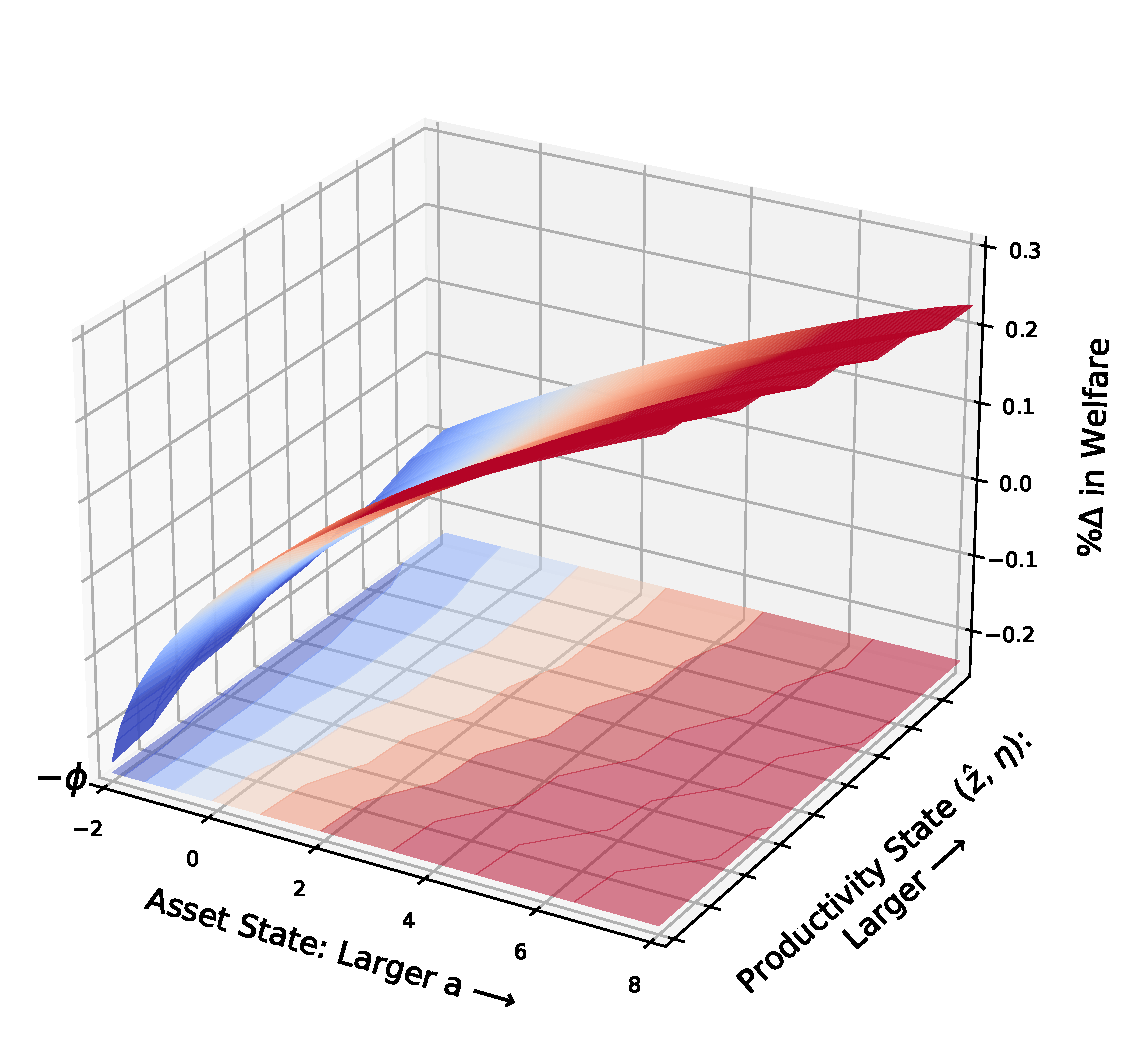
\includegraphics[scale = .45]{../notes/figures/welfare-aut.pdf}}
\end{figure}
\end{frame}


\begin{frame}[t]
\frametitle{U.S. Welfare: 10\% Reduction to a Small Market (Australia)}
\begin{table}[t]
\footnotesize
\setlength {\tabcolsep}{6.05mm}
\renewcommand{\arraystretch}{1.80}
\begin{center}
\begin{tabular}{l c c}
\multicolumn{3}{c}{\small \textbf{Welfare by Wealth --- Australia {\color{red} 10\%} Reduction}}\\
\hline
\hline
& \footnotesize  Fixed $R$ \& $w$ & GE: Prices Adjust \\
\cmidrule(lr){2-2}  \cmidrule(lr){3-3}
\footnotesize  Asset Quartile & \footnotesize  Welfare (\% Change) & \footnotesize  Welfare (\% Change) \\
\footnotesize  Bottom quartile  & 0.0013 & -0.163 \\
\footnotesize  Median & 0.0023 & -0.078 \\
\footnotesize  Upper quartile  & 0.0052 & 0.084  \\
\footnotesize  Aggregate & 0.0031 & -0.056  \\
\cmidrule(lr){2-2}  \cmidrule(lr){3-3}
\footnotesize  \% losers & 0.0 & 72.6\\
\hline
\end{tabular}
%\parbox[c]{3.65in}{\vspace{.1cm}
%{\footnotesize \textbf{Note:}}}
\end{center}
\end{table}
\end{frame}


%%%%%%%%%%%%%%%%%%%%%%%%%%%%%%%%%%%%%%%%%%%%%%%%%%%%%%%%%%%%%%%%%%%%%%%%%%%%%%%%%%%%%%%%%%%%%%%%%
%%%%%%%%%%%%%%%%%%%%%%%%%%%%%%%%%%%%%%%%%%%%%%%%%%%%%%%%%%%%%%%%%%%%%%%%%%%%%%%%%%%%%%%%%%%%%%%%%

\begin{frame}[t]{Micro-Elasticities I: The Intensive Margin}
\smallskip
How do households respond on the \textbf{intensive} margin to a change in trade costs?
\begin{align*}
\theta_{ij}(a,z)^{I} & := \frac{\partial c_{ij}(a,z)/ c_{ij}(a,z)}{\partial d_{ij} / d_{ij}}, \\
\\
& = \bigg [-\frac{\partial g_{ij}(a,z)/ p_{ij}c_{ij}(a,z)}{\partial p_{ij}/ p_{ij}} - 1 \bigg ]\frac{\partial p_{ij}/p_{ij}}{\partial d_{ij}/ d_{ij}}.
\end{align*}\\
\bigskip
\medskip
The idea: A reduction in trade costs relaxes the hh's budget constraint, so the intensive margin elasticity depends on the division of new resources between assets and expenditure.
\end{frame}

%%%%%%%%%%%%%%%%%%%%%%%%%%%%%%%%%%%%%%%%%%%%%%%%%%%%%%%%%%%%%%%%%%%%%%%%%%%%%%%%%%%%%%%%%%%%%%%%
%%%%%%%%%%%%%%%%%%%%%%%%%%%%%%%%%%%%%%%%%%%%%%%%%%%%%%%%%%%%%%%%%%%%%%%%%%%%%%%%%%%%%%%%%%%%%%%%

\begin{frame}[t]{Micro-Elasticities II: The Extensive Margin}
\smallskip
How do households respond on the \textbf{extensive} margin?
\begin{align*}
\theta_{ij}(a,z)^{E} &:= \frac{\partial \pi_{ij}(a,z) / \pi_{ij}(a,z)}{\partial d_{ij} / d_{ij}}, \\
\nonumber \\
& = - \frac{\partial \Phi_{i}(a,z) / \Phi_{i}(a,z)}{\partial d_{ij}/d_{ij}} -\frac{1}{\sigma_{\epsilon}}\bigg[u'(c_{ij}(a,z))c_{ij}(a,z)\bigg] + \beta \mathbb{E}\frac{1}{\sigma_{\epsilon}}\frac{\partial v_{i}(a',z')}{\partial d_{ij}/ d_{ij}}.
\end{align*}\\
\medskip
\bigskip
\uncover<2>{To get a sense of things, vary the second term by wealth\ldots
\begin{align*}
\frac{\partial (u'(c_{ij}(a,z))c_{ij}(a,z))}{\partial a} = u'(c_{ij}(a,z))\times \mathbf{MPC}_{ij}(a,z) \times \bigg[-\rho_{ij}(a,z) + 1\bigg],
\end{align*}\\
\medskip
where $\rho_{ij}(a,z)$ is the Arrow-Pratt measure of relative risk aversion.\\
\medskip
With CRRA, if risk aversion $> \ 1 \ $, then poor, high marginal utility households (who are also high MPC households) are \emph{more elastic relative} to rich households on the extensive margin.}
\end{frame}

%%%%%%%%%%%%%%%%%%%%%%%%%%%%%%%%%%%%%%%%%%%%%%%%%%%%%%%%%%%%%%%%%%%%%%%%%%%%%%%%%%%%%%%%%%%%%%%%
%%%%%%%%%%%%%%%%%%%%%%%%%%%%%%%%%%%%%%%%%%%%%%%%%%%%%%%%%%%%%%%%%%%%%%%%%%%%%%%%%%%%%%%%%%%%%%%%

\begin{frame}[t]{Bilateral Trade Elasticities: German Example}
\begin{figure}[!t]
\centering{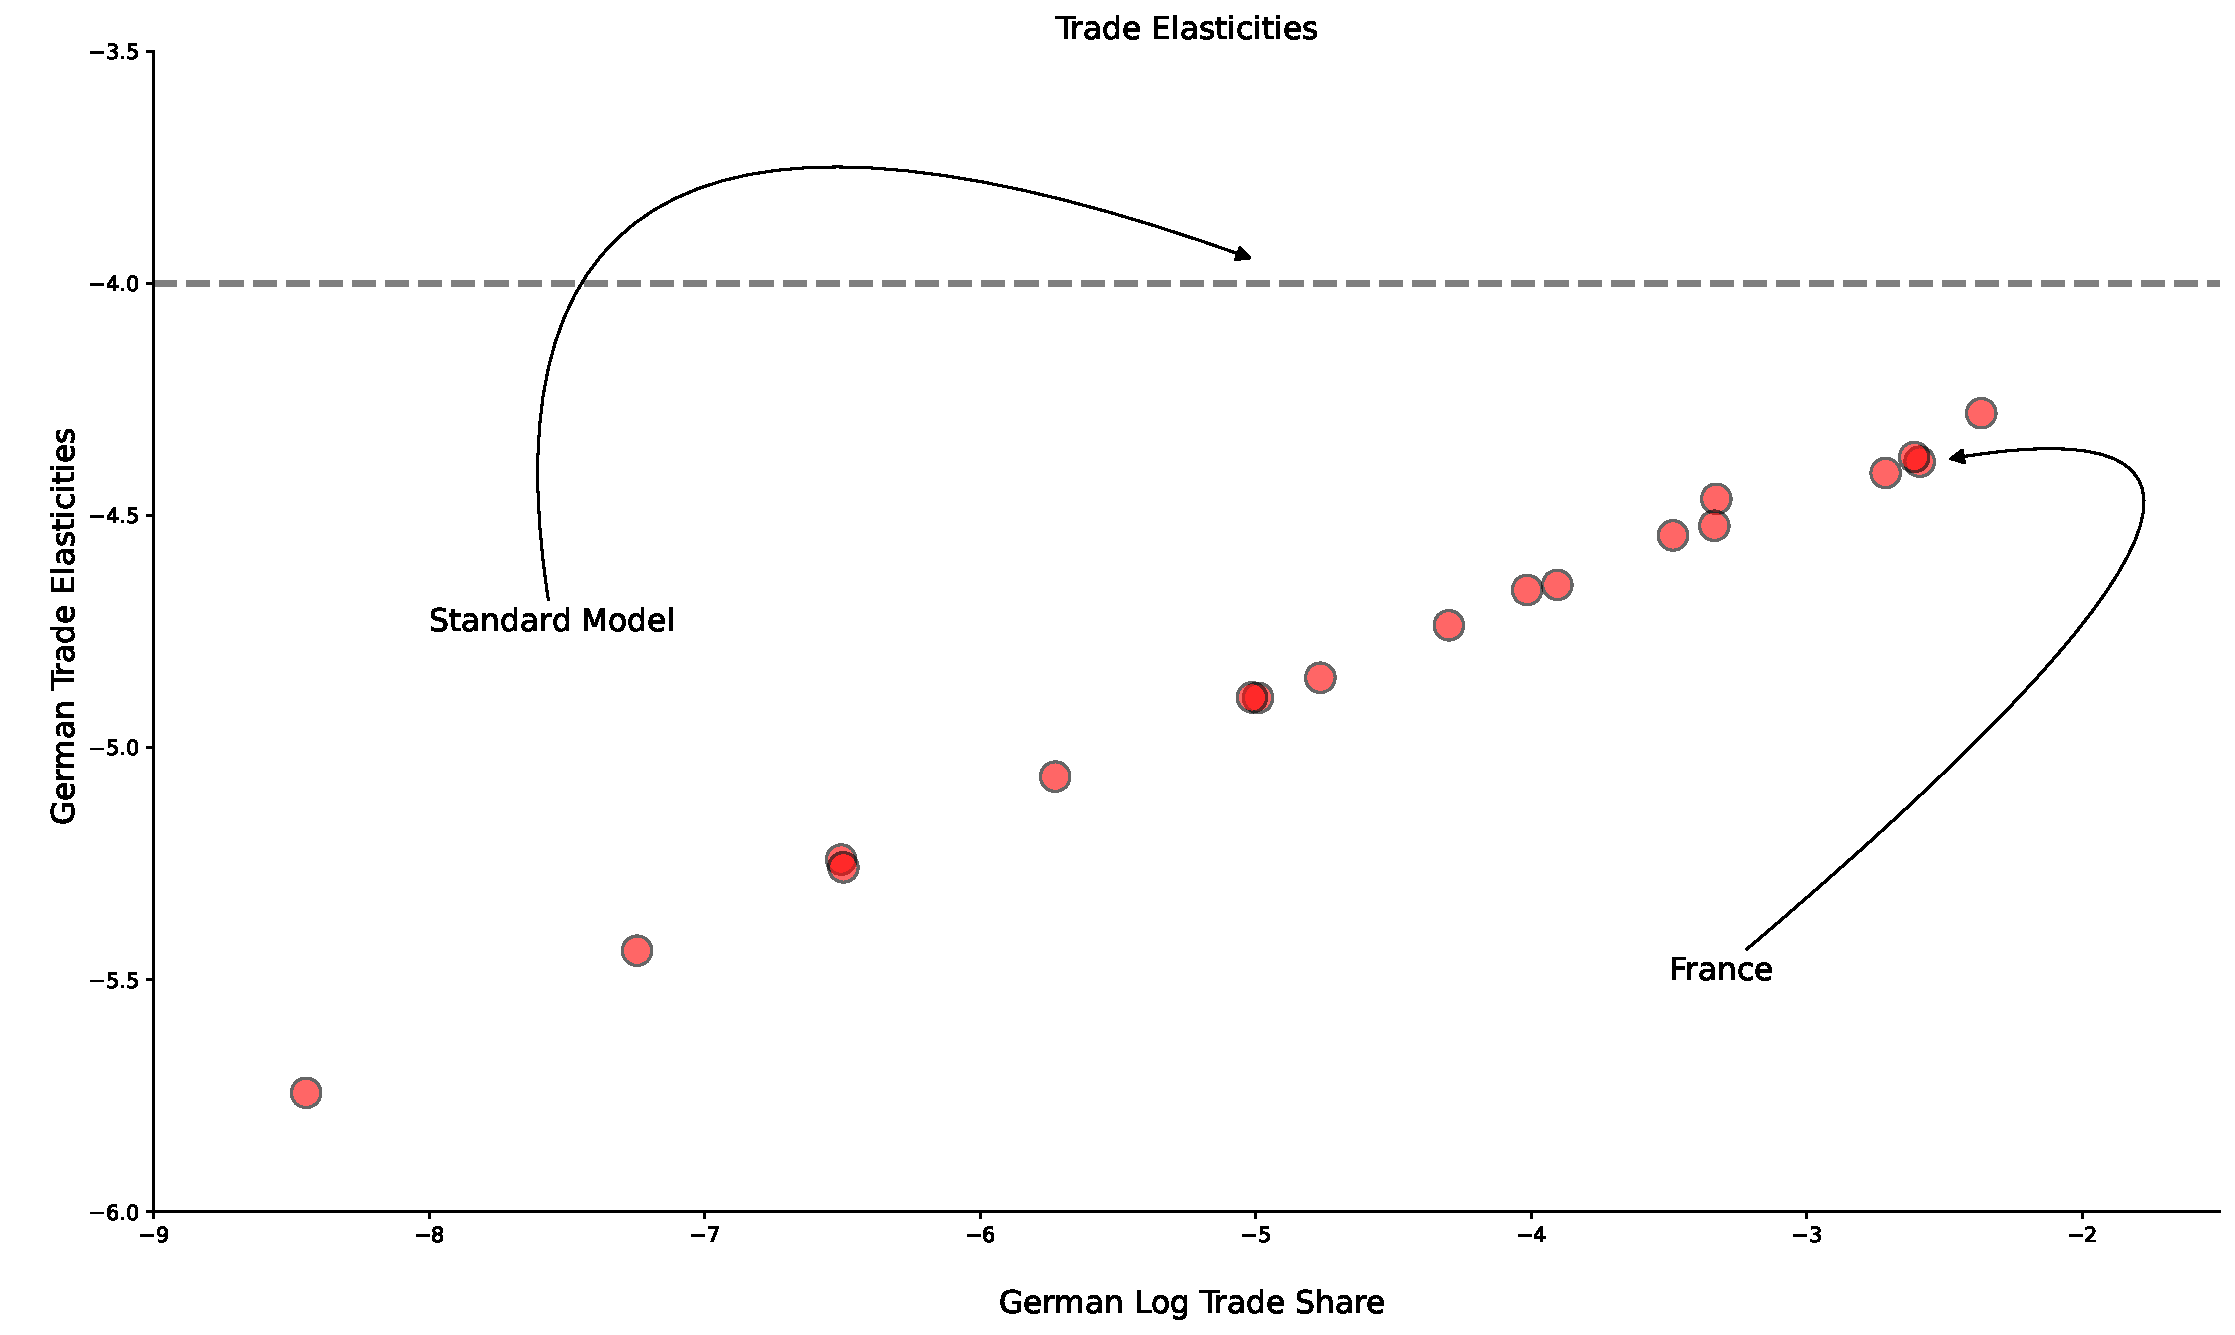
\includegraphics[scale = .35]{../notes/figures/german-trade-elasticities.pdf}}
\end{figure}
\end{frame}





\setcounter{framenumber}{\value{finalframe}}

%%%%%%%%%%%%%%%%%%%%%%%%%%%%%%%%%%%%%%%%%%%%%%%%%%%%%%%%%%%%%%%%%%%%%%%%%%%%%%%%%%%%%%%%%%%%%%%%%
%%%%%%%%%%%%%%%%%%%%%%%%%%%%%%%%%%%%%%%%%%%%%%%%%%%%%%%%%%%%%%%%%%%%%%%%%%%%%%%%%%%%%%%%%%%%%%%%%



\end{document} 